\documentclass[acmsmall,screen,review,anonymous]{acmart}

\AtBeginDocument{%
  \providecommand\BibTeX{{%
    Bib\TeX}}}

\usepackage{graphicx}
\usepackage{subcaption}
\usepackage{amsmath}
\usepackage{amsfonts}
\usepackage{enumitem}
\usepackage{tcolorbox}
\usepackage{multirow}
\usepackage{xcolor}
\usepackage{colortbl}
\usepackage{array}
\usepackage{tabularx}
\usepackage{makecell}
\usepackage{pifont}
\usepackage{pgf}
\usepackage{booktabs}
\tcbuselibrary{listings,skins,breakable}  % 关键：支持 listings 和跨页

%\usepackage[draft,commandnameprefix=ifneeded]{changes}
% \usepackage[final,commandnameprefix=ifneeded]{changes} % draft for revised version, and final for final verision

\usepackage{listings}
% 自定义 Markdown 语言，避免特殊字符冲突
\lstdefinelanguage{Markdown}{
  alsoletter={\#\*\-\+\_},
  morecomment=[l]{<!--},
  % morestring=[b]",
  % morestring=[b]',
  sensitive=false
}

\definecolor{MyPicBlue}{HTML}{EBF4FF}
\definecolor{MyPicBorder}{HTML}{B3D7FF}
% 定义一个名为 SummaryBox 的新环境
\newtcolorbox{SummaryBox}{
    colback=MyPicBlue,       % 框内背景颜色
    colframe=MyPicBorder,      % 边框颜色
    arc=2pt,               % 圆角弧度（如果不想要圆角，可以改为 0pt）
    boxrule=0.5pt,         % 边框粗细
    left=2pt, right=2pt,   % 左右内边距
    top=2pt, bottom=2pt,   % 上下内边距
    % before=\vspace{0.5em},  % 框前垂直间距
    % after=\vspace{0.5em}    % 框后垂直间距
}

% 自定义 Markdown 样式
\lstdefinestyle{markdown-style}{
  language=Markdown,
  backgroundcolor=\color{green!2},
  basicstyle=\ttfamily\scriptsize,
  keepspaces=true,
  keywordstyle=\color{blue}\bfseries,
  commentstyle=\color{gray},
  stringstyle=\color{red},
  breaklines=true,
  breakindent=0pt,
  postbreak=,
  showstringspaces=false,
  columns=fullflexible,
}

\newtcblisting{markdowncode}{
  breakable,                  % 支持跨页（双栏中也更稳定）
  enhanced,                   % 支持高级 TikZ 效果
  colback=green!2,            % 背景色（您原代码块是 green!2，这里统一）
  colframe=blue!70!black,     % 边框颜色
  boxrule=1pt,                % 边框粗细（可调整）
  arc=10pt,                   % 圆角 10pt（所有角）
  sharp corners=east,         % 右边三个角变方角，只左边圆角（完美匹配您的 leftline=true, rightline=false）
  % left=4pt, right=4pt, top=4pt, bottom=4pt,  % 内边距（可微调）
  leftrule=0pt,               
  toprule=0pt, bottomrule=0pt, rightrule=0pt, % 隐藏上、下、右边线
  % titlerule=0pt,              % 无标题时隐藏标题线
  fontlower=\small,           % 内容字体（对应您的 font=\small）
  % top=2ex, bottom=1ex,        % 框上方/下方间距（对应 skipabove/skipbelow）
  listing only,               % 只显示 listings 内容
  listing options={style=markdown-style},
}

\lstdefinestyle{artifact-style}{
  language=Markdown,
  backgroundcolor=\color{yellow!5},
  basicstyle=\ttfamily\scriptsize,
  keepspaces=true,
  keywordstyle=\color{blue}\bfseries,
  commentstyle=\color{gray},
  stringstyle=\color{red},
  breaklines=true,
  breakindent=0pt,
  postbreak=,
  showstringspaces=false,
  columns=fullflexible,
}

\newtcblisting{artifact}{
  breakable,                  % 支持跨页（双栏中也更稳定）
  enhanced,                   % 支持高级 TikZ 效果
  colback=yellow!5,            % 背景色（您原代码块是 green!2，这里统一）
  colframe=blue!70!black,     % 边框颜色
  boxrule=1pt,                % 边框粗细（可调整）
  arc=10pt,                   % 圆角 10pt（所有角）
  sharp corners=east,         % 右边三个角变方角，只左边圆角（完美匹配您的 leftline=true, rightline=false）
  % left=4pt, right=4pt, top=4pt, bottom=4pt,  % 内边距（可微调）
  leftrule=0pt,               
  toprule=0pt, bottomrule=0pt, rightrule=0pt, % 隐藏上、下、右边线
  % titlerule=0pt,              % 无标题时隐藏标题线
  fontlower=\small,           % 内容字体（对应您的 font=\small）
  % top=2ex, bottom=1ex,        % 框上方/下方间距（对应 skipabove/skipbelow）
  listing only,               % 只显示 listings 内容
  listing options={style=artifact-style},
}
\newcommand{\ourtool}{RAFT}
\newcommand{\strategy}{Adaptive Purification-Aggregation}
\newcommand{\strategymm}{Purification}
\newcommand{\strategyrr}{Aggregation}
\newcolumntype{L}{>{\raggedright\arraybackslash}X}
\newcolumntype{Y}{>{\centering\arraybackslash}X}
\citestyle{acmnumeric}
\setlength{\textfloatsep}{8pt plus 2pt minus 2pt}
\setlength{\floatsep}{8pt plus 2pt minus 2pt}
\setlength{\intextsep}{8pt plus 2pt minus 2pt}
\captionsetup{skip=4pt}

\setcopyright{none}
\acmDOI{}
\acmISBN{}
\renewcommand\footnotetextcopyrightpermission[1]{}

\begin{document}


%\title{Distilling Tacit Regulatory Knowledge from LLMs to Auto-Formalize Requirements for Compliance Test Case Generation}

%\title{Distilling Formal Models from LLMs for Automatic  Model-Based Compliance Testing}

\title{Explicating Implicit Regulatory Knowledge in LLMs for Automatic Compliance Test Case Generation}


\author{Anonymous Author(s)}
% \author{Ben Trovato}
% \authornote{Both authors contributed equally to this research.}
% \email{trovato@corporation.com}
% \orcid{1234-5678-9012}
% \author{G.K.M. Tobin}
% \authornotemark[1]
% \email{webmaster@marysville-ohio.com}
% \affiliation{%
%   \institution{Institute for Clarity in Documentation}
%   \city{Dublin}
%   \state{Ohio}
%   \country{USA}
% }

% \author{Lars Th{\o}rv{\"a}ld}
% \affiliation{%
%   \institution{The Th{\o}rv{\"a}ld Group}
%   \city{Hekla}
%   \country{Iceland}}
% \email{larst@affiliation.org}

% \author{Valerie B\'eranger}
% \affiliation{%
%   \institution{Inria Paris-Rocquencourt}
%   \city{Rocquencourt}
%   \country{France}
% }

% \author{Aparna Patel}
% \affiliation{%
%  \institution{Rajiv Gandhi University}
%  \city{Doimukh}
%  \state{Arunachal Pradesh}
%  \country{India}}

% \author{Huifen Chan}
% \affiliation{%
%   \institution{Tsinghua University}
%   \city{Haidian Qu}
%   \state{Beijing Shi}
%   \country{China}}

% \author{Charles Palmer}
% \affiliation{%
%   \institution{Palmer Research Laboratories}
%   \city{San Antonio}
%   \state{Texas}
%   \country{USA}}
% \email{cpalmer@prl.com}

% \author{John Smith}
% \affiliation{%
%   \institution{The Th{\o}rv{\"a}ld Group}
%   \city{Hekla}
%   \country{Iceland}}
% \email{jsmith@affiliation.org}

% \author{Julius P. Kumquat}
% \affiliation{%
%   \institution{The Kumquat Consortium}
%   \city{New York}
%   \country{USA}}
% \email{jpkumquat@consortium.net}

\begin{abstract}
Generating regulatory compliance test cases remains labor-intensive because
regulations must be interpreted and connected to system behavior. Existing
hybrid LLM and model-based approaches improve automation and structure but
often require manually engineered domain knowledge. We present RAFT, which
keeps input regulations authoritative for rule-level semantics while
explicating implicit regulatory knowledge in LLMs into three reusable
meta-level artifacts: a domain meta-model, a requirements representation, and
testability constraints. LLMs construct these
artifacts from parametric knowledge, optionally supported by a small corpus,
and RAFT injects them into requirements formalization, testability assessment,
and test generation. Across 11 financial, road-traffic, and power datasets,
RAFT attains 91.7\% F1 and 87.1\% business scenario coverage in finance. Its
observed F1 is 23.6 points above the strongest automated baseline and favors
RAFT on all six financial datasets. Fully automated RAFT takes 2.53 hours;
artifact review raises F1 to 96.2\% in 5.03 hours of elapsed time and requires 7.16
person-hours, versus 42.56 measured person-hours for expert-authored reference
cases. Together, these results indicate that RAFT provides a practical
path to scalable, knowledge-guided compliance test generation.

% introduce an Adaptive Purification-Aggregation strategy that, observing that these artifacts exhibit opposite failure modes, adaptively consolidates the LLM outputs to keep them robust and complete.

%To reduce this reliance and minimize human expert intervention, in this paper we propose a novel framework called RAFT, for automated requirements formalization and compliance test generation via .

\end{abstract}

\begin{CCSXML}
<ccs2012>
<concept>
<concept_id>10011007.10011074.10011099.10011102.10011103</concept_id>
<concept_desc>Software and its engineering~Software testing and debugging</concept_desc>
<concept_significance>500</concept_significance>
</concept>
<concept>
<concept_id>10011007.10011074.10011075.10011076</concept_id>
<concept_desc>Software and its engineering~Requirements analysis</concept_desc>
<concept_significance>300</concept_significance>
</concept>
</ccs2012>
\end{CCSXML}

\ccsdesc[500]{Software and its engineering~Software testing and debugging}
\ccsdesc[300]{Software and its engineering~Requirements analysis}


\keywords{Software compliance testing, Requirements engineering, Large language models, Model-based testing}


% \received{20 February 2007}
% \received[revised]{12 March 2009}
% \received[accepted]{5 June 2009}

\maketitle


\section{Introduction}
\label{sec:introduction}

Software in regulated domains such as finance, automotive, and power must
conform to extensive regulations, standards, and internal
policies~\cite{badrzadeh2015challenges,tabani2019assessing,xue2024llm4fin,zhang2025comprehensive}.
Regulatory compliance testing provides a final opportunity to detect
violations before deployment~\cite{sommerville2005ingenieria}. Yet producing
these tests remains largely manual: experts must interpret regulatory
documents, formalize implicit conditions, and connect test cases to
system interfaces~\cite{castellanos2022compliance,jain2025complexity}.
Regulations also contain cross-rule dependencies and context-sensitive
terminology rather than isolated requirements. A usable workflow must therefore
preserve source provenance, represent pre- and post-operation states, and
compose related rules into structured test scenarios.

Model-based approaches derive tests from domain models, graphs, or formal
representations and offer interpretability and controllability, but adapting
their artifacts can require substantial engineering
effort~\cite{wang2022automatic,stefani2025automated,zyberaj2025genai,yang2025llmcfg}.
LLM-based approaches automate more of the process through prompting,
retrieval-augmented generation, or multi-agent
collaboration~\cite{lewis2020retrieval,castellanos2022compliance,boukhlif2024towards,korraprolu2025test,hasan2025automatic,masuda2026generating},
but can produce hallucinated or inconsistent outputs. Hybrid methods guide
LLMs with ontologies, schemas, or formal specifications, improving structure
while still depending on manually constructed domain
knowledge~\cite{xue2024llm4fin,chen2024automated,sun2025compliance,shrestha2025less}.

The bottleneck therefore shifts from test generation to reusable knowledge
construction. The challenge is not simply a lack of domain facts. Direct
generation collapses rule interpretation, representation choice, and test
design into one opaque output, making errors difficult to localize and
improvements difficult to reuse. At the other extreme, manually engineered
artifacts improve control but must be rebuilt and maintained for each domain.
We therefore need an explicit boundary between authoritative rule semantics and
reusable generation guidance. This raises two questions: which intermediate representation is
structured enough for downstream testing, and how can its supporting domain
knowledge be obtained without recreating the same manual burden? We use formal
requirements because they balance expressiveness, machine interpretability,
and testability~\cite{gropler2021nlp,yang2025requirements}.

We address this bottleneck with \ourtool, a framework for
\underline{R}equirements \underline{A}uto-\underline{F}ormalization and
Compliance \underline{T}est Generation. \ourtool\ separates two knowledge
layers. The input regulation remains authoritative for rule-level obligations,
thresholds, and exceptions. Implicit regulatory knowledge in LLMs is explicated
into three reusable meta-level artifacts: a domain meta-model, a requirements
representation, and testability constraints. A small construction
corpus of documents and historical tests is optional and supplies evidence
about scope, terminology, granularity, and output format. \ourtool\ injects
these artifacts at the corresponding stages to formalize regulations, assess
testability, and generate compliance test cases. The meta-model
defines domain concepts, relations, operations, and state fields; the
requirements representation defines a constrained \textit{KEY-OP-VALUE}
grammar; and the testability artifact defines OCL-style decision predicates.
Generated formal requirements retain source-rule evidence and explicitly
encode their pre- and post-operation states. Knowledge construction is
completed and frozen before evaluation documents enter the generation phase,
preventing held-out rule content from leaking into the reusable artifacts.
This layered design makes errors attributable to vocabulary, formalization,
testability, or generation and permits artifact inspection and correction
without changing the authoritative rule text.

\ourtool\ constructs candidates with multiple LLMs and applies an \strategy\
strategy. Purification retains majority-supported meta-model elements, whereas
aggregation preserves complementary representation and testability knowledge.
The assignment follows artifact-specific failure costs: unsupported meta-model
elements can corrupt downstream stages, while deleting valid representation or
testability knowledge reduces coverage. Artifacts and provenance are retained
for inspection.

We evaluate \ourtool\ on 11 financial, road-traffic, and power datasets. The
controlled E2E baseline matches backends and documents but omits explicit
artifacts. On six financial datasets, \ourtool\ achieves 91.7\% F1/87.1\% BSC,
23.6 F1 points above the strongest automated baseline and higher on every
dataset; HITL reaches 96.2\% F1. Automated \ourtool, HITL, and experts require
2.53 elapsed hours, 5.03 elapsed hours (7.16 person-hours), and 42.56
person-hours. Secondary analyses show 90.2\% corpus-free F1, gains from explicit
artifacts and operator assignment, wins on 10 of 11 backbones, and
re-instantiated F1 of 92.7\%/87.2\% in road traffic/power.

Beyond the metric gains, \ourtool\ turns transient model outputs into reusable
engineering assets. Explicit artifact contracts make knowledge inspectable and
traceable, support targeted revision before generation, and provide stable
interfaces across changing regulations, models, and domains. This design
supports repeated compliance workflows and incremental maintenance. Because the
artifacts are decoupled from individual rules, teams can reuse them across
document revisions and compare outputs across LLM backbones. Their shared
structure also gives engineers and domain experts a common review surface.

Together, these results show the practical value of reusable, inspectable
artifacts for compliance test generation.

The contributions of this paper are:
\begin{enumerate}[leftmargin=*,align=left,label=(\arabic*), itemsep=0pt, parsep=0pt, nosep]
    \item \textbf{Automated Compliance-Test Framework.}
    \ourtool\ separates authoritative rule semantics from reusable artifacts
    for traceable formalization, testability assessment, and test generation.

    \item \textbf{Risk-Adaptive Knowledge Explication.}
    Our \strategy\ strategy assigns purification or aggregation by artifact type
    to consolidate three complementary artifacts from multiple LLM outputs.

    \item \textbf{Cross-Domain Evaluation.}
    We evaluate three domains with ablations, expert review, step-level and
    backbone analyses, and a shared cost, time, and run-variation protocol.
\end{enumerate}

\section{Related Work}
\label{sec:related_work}

% Test case generation from natural-language documents has evolved along three paradigms, model-based, LLM-based, and hybrid, as illustrated in Figure~\ref{fig:related_work}. We review these paradigms and their application to regulatory compliance testing.

\subsection{Test Generation from Natural-Language Requirements}

Test generation from natural-language requirements follows three broad paradigms. \textit{Model-based methods} derive tests from explicit behavioral or structural representations, including control-flow graphs~\cite{yang2025llmcfg}, system graphs~\cite{zyberaj2025genai}, Operational Design Domain models~\cite{stefani2025automated}, and domain-specific models for financial systems~\cite{jin2019finexpert}. These representations support systematic generation and inspection, but creating or adapting them often requires domain-specific modeling effort~\cite{xue2024domain}.

\textit{LLM-based methods} generate test specifications directly from requirements through prompt engineering and prompt chaining~\cite{masuda2026generating,bhatia2024system,boukhlif2024towards}, or decompose the task into multiple generation stages~\cite{milchevski2025multi}. Comparative and industrial studies report improved automation but also expose sensitivity to prompts, models, and requirement complexity~\cite{hasan2025automatic,korraprolu2025test,wang2025testeval,zhang2024testbench}.

\textit{Hybrid methods} combine LLMs with explicit domain artifacts. Examples include domain-model-guided financial acceptance testing~\cite{xue2024llm4fin}, ontology-guided BIM compliance checking~\cite{chen2024automated}, retrieval-grounded compliance checking~\cite{sun2025compliance}, and test generation from formal requirements~\cite{shrestha2025less}. These artifacts improve structure and controllability, but when they are manually engineered, adaptation shifts effort from test generation to knowledge construction and maintenance.


% Model-based approaches derive test cases from intermediate behavioral or structural models, such as graphs, domain models, and formal specifications, via techniques like graph traversal, symbolic execution, and constraint solving. For instance, Yang et al. construct Control Flow Graphs (CFGs) from requirements and enumerate executable paths~\cite{yang2025llmcfg}, Zyberaj et al. transform specifications into System Graphs (SGs) for test generation~\cite{zyberaj2025genai}, and in safety-critical domains, Operational Design Domain (ODD) models and formal representations are used to capture regulatory constraints for testing~\cite{stefani2025automated,jin2019finexpert}. Such explicit modeling offers strong interpretability and controllability, but building and maintaining the models demands substantial expertise, raising cost and limiting portability across domains~\cite{xue2024domain}.


% Model-based approaches generate test cases by first transforming the rules or requirements into intermediate models, such as graphs, domain models, or formal representations, and then applying algorithmic analysis such as traversal and constraint solving.
% For example, Yang et al. construct Control Flow Graphs (CFG) from requirements and generate test cases by enumerating executable paths \cite{yang2025llmcfg}.
% Zyberaj et al. convert system specifications into structured System Graphs (SG), from which executable scenarios are derived to support efficient test case generation \cite{zyberaj2025genai}.
% In safety-critical domains, researchers further employ domain-specific models, such as Operational Design Domain (ODD) models and Formal Representations (FR), to encode regulatory knowledge, constraints, and requirements, and to support subsequent compliance test case generation \cite{stefani2025automated,jin2019finexpert}.

% While model-based approaches offer strong controllability and interpretability, they rely on manual or rule-based NLP tools to construct intermediate models. Building and maintaining such models requires substantial domain expertise and engineering effort, thereby limiting scalability in real-world settings \cite{xue2024domain}.



% \vspace{1mm}
% \noindent
% \textbf{LLM-Based Test Generation.}
% LLM-based methods generate test cases from natural-language requirements, specifications, or regulations using LLMs. Prompt-based methods guide LLMs via prompt engineering or chaining, e.g., extracting test design techniques before generation~\cite{masuda2025generating} or chaining prompts to produce structured test artifacts~\cite{bhatia2024system}. Agent-based methods decompose generation into coordinated stages to simulate professional testing workflows~\cite{milchevski2025multi} or stress testing and diagnosis~\cite{jin2025guard}. Domain adaptation via RAG, supervised fine-tuning (SFT), and reinforcement learning (RL) has also been explored~\cite{boukhlif2024towards,hasan2025automatic}. These methods improve automation and flexibility, yet LLM stochasticity leaves them prone to hallucinations and inconsistent outputs, limiting reliability in safety-critical compliance testing~\cite{wang2025testeval,korraprolu2025test,zhang2024testbench}.


% LLM-based approaches generate test cases directly from natural language requirements, either via prompt engineering or agent frameworks.

% Prompt-based approaches rely on prompt engineering to guide LLMs in test generation. Masuda et al. extract test design techniques before generating high-level test cases~\cite{masuda2025generating}. 
% Bhatia et al. employ prompt chaining to produce structured test tables from full documents~\cite{bhatia2024system}. 
% Despite their simplicity and flexibility, these methods suffer from limited reliability: they struggle to target specific execution branches and degrade on complex requirements due to insufficient reasoning and lack of domain knowledge~\cite{wang2025testeval,korraprolu2025test}.

% Agent-based systems address these limitations by decomposing test generation into coordinated stages. 
% Milchevski et al. design a multi-agent framework that simulates professional testing workflows, including requirements analysis, test design, and generation~\cite{milchevski2025multi}. 
% Jin et al. adopt multi-LLM orchestration for stress testing and diagnostic analysis~\cite{jin2025guard}. 
% While RAG and fine-tuning have been explored for domain integration ~\cite{boukhlif2024towards,hasan2025automatic}, these approaches remain limited by LLM stochasticity, leading to hallucinations, unstable outputs, and incomplete coverage of critical program behaviors\cite{zhang2024testbench,korraprolu2025test}.

% \vspace{1mm}
% \noindent
% \textbf{Hybrid Frameworks.}
% Hybrid approaches guide LLMs with domain knowledge artifacts, such as ontologies, schemas, templates, or formal specifications, to construct intermediate representations that support test generation. For example, Xue et al. use a domain meta-model to guide LLM-based information extraction and combine it with scenario synthesis for financial compliance testing~\cite{xue2024llm4fin}, Chen et al. embed domain ontologies into an LLM-assisted pipeline for compliance checking in BIM~\cite{chen2024automated}, and others apply requirement templates or formal schemas to constrain generation~\cite{sun2025compliance,shrestha2025less}. Such grounding improves reliability and controllability, but the artifacts are typically hand-engineered and costly to maintain when adapting to new regulations or domains, shifting the bottleneck from test generation to knowledge engineering.


% Hybrid approaches aim to bridge the gap between the above two methods by using LLMs to construct intermediate models, guided and constrained by domain knowledge such as ontologies, schemas, or formal specifications. These intermediate models are then leveraged for test generation.
% For example, Xue et al. define a domain meta-model to guide LLM-based information extraction and integrate it with rule-driven scenario synthesis, enabling automated test case generation from business rules~\cite{xue2024llm4fin}.
% Chen et al. incorporate domain ontologies into an LLM-assisted pipeline for compliance checking in BIM, enabling more precise interpretation of regulatory texts \cite{chen2024automated}.
% Other approaches adopt RAG or requirement templates to further constrain LLM outputs~\cite{sun2025compliance,shrestha2025less}.

% Although grounding LLM generation in domain knowledge mitigates hallucinations, manual knowledge construction limits scalability and adaptability, necessitating automated methods that reduce human involvement and enable generalizable test generation.



\subsection{Regulatory Compliance Testing}
Compliance testing has attracted growing attention in regulated settings. Earlier work formalizes regulations using controlled natural language, knowledge representations, and SBVR models~\cite{roychoudhury2018case,kholkar2016natural,roychoudhury2017natural}. More recent systems address financial acceptance-test generation with domain models~\cite{xue2024llm4fin}, retrieval-grounded regulatory compliance checking~\cite{sun2025compliance}, and formal-requirement-guided test generation~\cite{shrestha2025less}; adjacent industrial work assesses software adherence to automotive safety standards~\cite{tabani2019assessing}. These studies address different downstream tasks but commonly depend on domain-specific regulatory artifacts. \ourtool\ instead automates reusable meta-level artifact construction while keeping regulatory text authoritative.





\subsection{Knowledge Extraction from LLMs}
A growing body of work treats LLMs as queryable knowledge sources. Petroni et al.~\cite{petroni2019language} showed with the LAMA probe that pre-trained models can recall factual knowledge without fine-tuning. Subsequent probing- and prompting-based methods extract factual triples~\cite{jiang2020can,alivanistos2022prompting} or construct knowledge graphs at scale~\cite{bian2025llm}, although the extracted knowledge is often sensitive to prompt design and difficult to verify~\cite{youssef2023give}. These methods primarily target generic knowledge represented as triples or general-purpose graphs, whereas compliance testing requires domain-specific conceptual, representational, and testability artifacts. \ourtool\ therefore constructs candidate meta-level artifacts with multiple LLMs and consolidates them through artifact-specific purification or aggregation.

\begin{figure*}[!t]
    \centering
    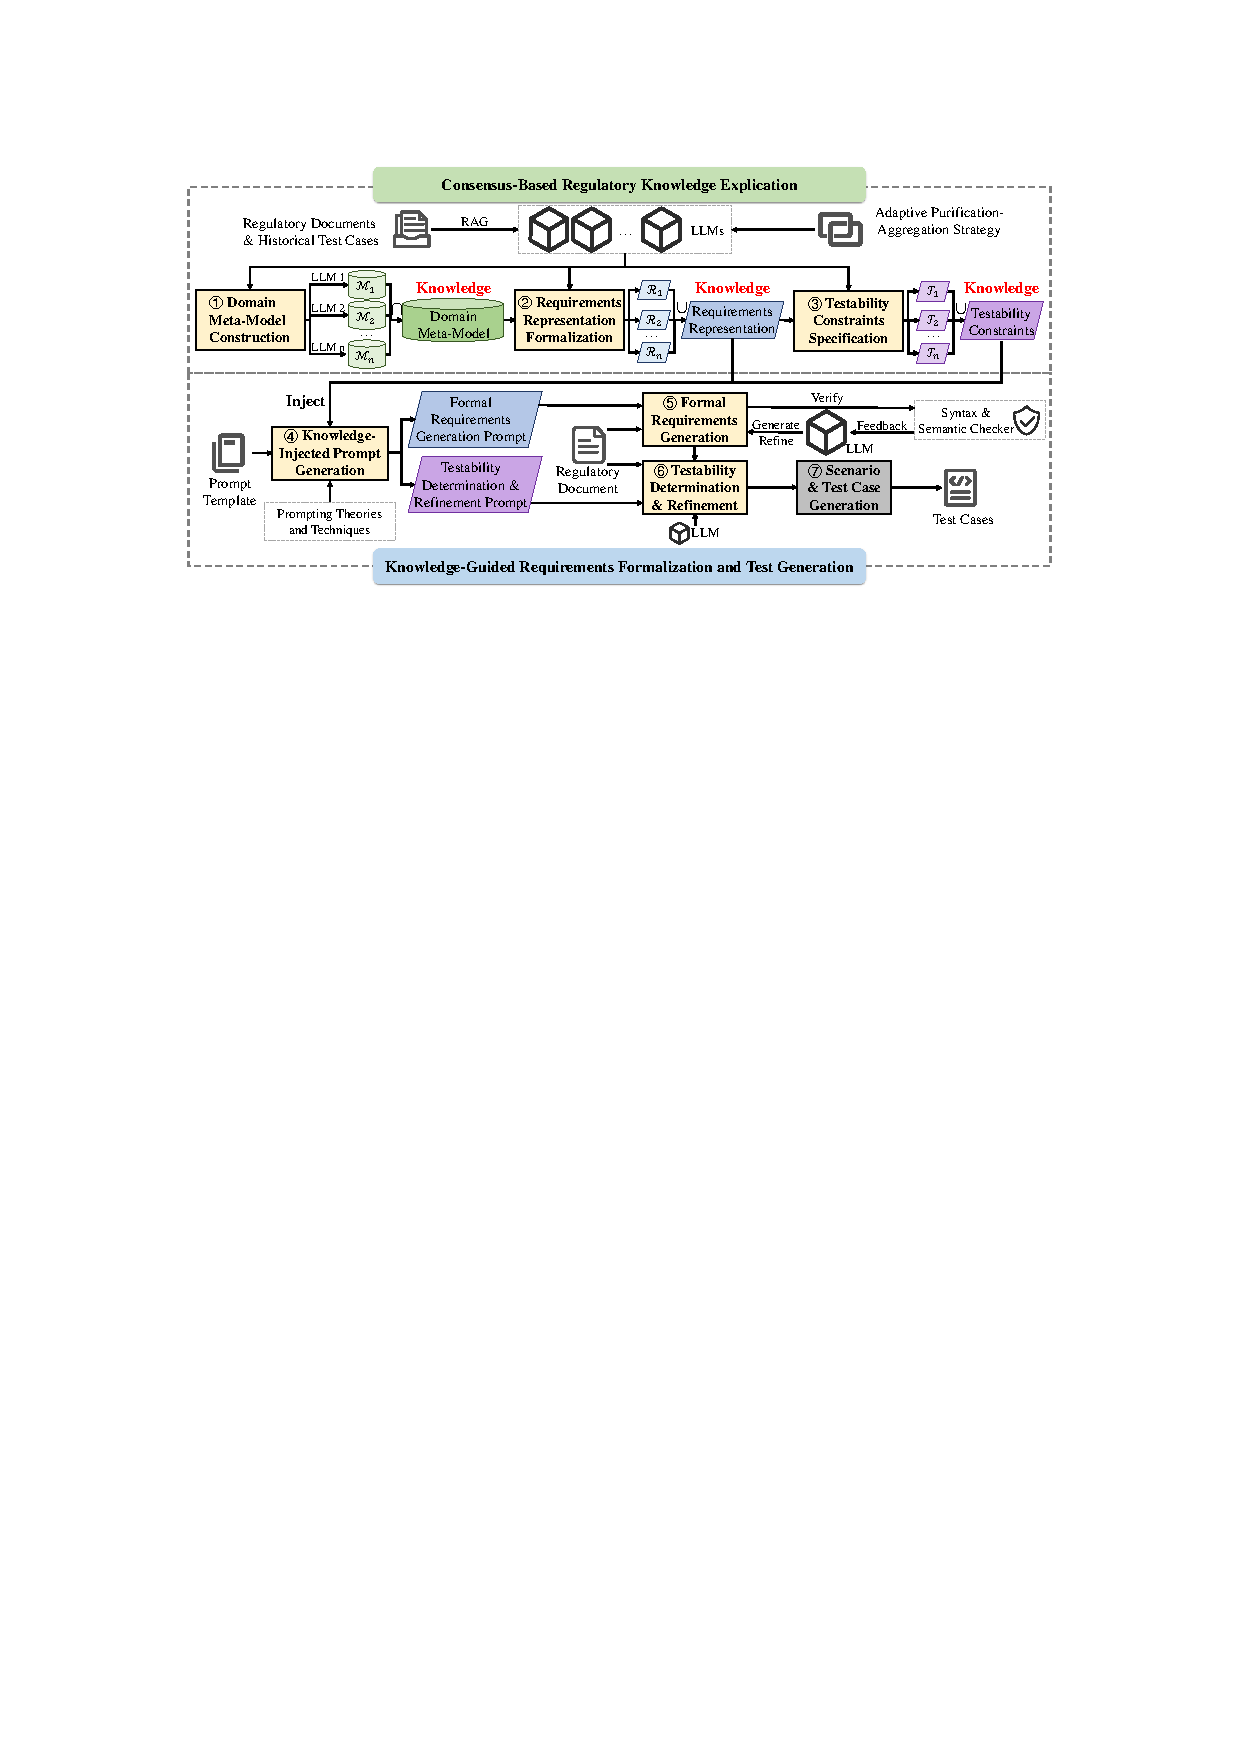
\includegraphics[width=0.9\linewidth]{fig/framework.pdf}
    \caption{\ourtool's knowledge-explication and knowledge-injected test-generation workflow.}
    \label{fig:framework}
    \Description{The RAFT workflow first explicates a domain meta-model, requirements representation, and testability constraints, then injects them into requirements formalization, testability refinement, and test generation.}
\end{figure*}

\section{The RAFT Approach}
\label{sec:method}


\subsection{Regulatory Knowledge and Framework Overview}




% To reduce reliance on manual effort in hybrid frameworks, a key challenge is automatically deriving and constructing knowledge to guide intermediate model generation. 
% To this end, we first consider the choice of an appropriate intermediate model. Among various alternatives, we adopt \textit{Formal Requirements}, as they (i) preserve the semantics of natural language rules, and (ii) provide a structured representation suitable for subsequent test generation \cite{gropler2021nlp,yang2025requirements}.

% Given this target, the required knowledge should enable LLMs to generate valid and testable formal requirements. 
% This involves three essential aspects: (i) the fundamental entities involved, (ii) the rules for composing these entities into valid structures, and (iii) the conditions under which formal requirements are testable.
% Accordingly, we define three complementary types of knowledge:
% \begin{enumerate}[leftmargin=*,align=left,label=(\arabic*), itemsep=0pt, parsep=0pt, nosep]
%     \item \textbf{Domain-Specific Meta Model ($\mathcal{M}$)}, which defines the core entities and semantic primitives of formal requirements.
%     \item \textbf{Requirements Representation ($\mathcal{R}$)}, which specifies the symbols, a data dictionary defining their types and value ranges \cite{silberschatz2002database}, and syntactic rules for constructing valid requirements.
%     \item \textbf{Testability Constraints ($\mathcal{T}$)}, which characterize the conditions under which the requirements are considered testable.
% \end{enumerate}
% Together, these components form a unified knowledge system that supports intermediate model generation.
% In the context of compliance testing, we collectively refer to them as \textit{Regulatory Knowledge}.


% Given that LLMs have internalized extensive regulatory knowledge through pretraining, this knowledge remains largely tacit and difficult to leverage \cite{zhang2023large,lu2025tacit}. To bridge this gap, we propose explicating such tacit knowledge into the three explicit artifacts: $\mathcal{M}$, $\mathcal{R}$, and $\mathcal{T}$, and dynamically injecting them into prompt templates to guide LLMs in two tasks: (1) transforming natural language rules into formal requirements, and (2) determining their testability.
% Testable requirements are then used to generate test cases via algorithms.

% In general, we propose \ourtool, a hybrid framework shown in Figure~\ref{fig:framework}, consisting of two phases:


% \textbf{Phase I: Regulatory Knowledge Explication.}
% The meta-model $\mathcal{M}$, requirements representation $\mathcal{R}$, and testability constraints $\mathcal{T}$ are automatically explicated from LLMs, transforming tacit knowledge into explicit and structured artifacts.

% \textbf{Phase II: Prompt and Test Case Generation.}
% The explicated artifacts are dynamically injected into prompt templates to guide requirements generation and testability determination, followed by test case generation, enabling an end-to-end automated workflow.

% The framework is designed to operate in an automated manner by default, while also supporting human-in-the-loop validation when necessary. All intermediate artifacts, such as knowledge artifacts and formal requirements, are stored and can be optionally reviewed and refined in safety-critical or high-assurance settings.


To transform regulations without manual modeling, we use \emph{formal
requirements} that encode domain concepts and behavioral constraints under a
grammar suitable for downstream analysis and generation~\cite{gropler2021nlp,yang2025requirements}.
``Formal'' denotes vocabulary and grammar conformance together with typed,
traceable state and constraint structures for downstream test generation. Each
requirement defines constraints over a pre-operation state, an operation, and
an expected post-operation state, and records its source-rule identifier and
supporting evidence. The downstream generator uses this abstract structure to
derive test cases with inputs, actions, and expected outcomes; an optional
adapter maps their fields to concrete interfaces for automated execution.

The knowledge comprises:
\begin{enumerate}[leftmargin=*,align=left,label=(\arabic*), itemsep=0pt, parsep=0pt, nosep]

\item \textbf{Domain Meta-Model ($\mathcal{M}$):}
the core domain entities and relations used in formalization.

\item \textbf{Requirements Representation ($\mathcal{R}$):}
the symbols, data types, value ranges, syntactic rules, and operational
conventions for constructing and processing valid formal
requirements~\cite{silberschatz2005database}.

\item \textbf{Testability Constraints ($\mathcal{T}$):}
formally stated OCL-style contexts, predicates, and invariants specifying the
conditions under which a formal requirement can be tested. Their semantic
predicates are assessed by LLMs rather than executed by an OCL engine.

\end{enumerate}
Together, they are explicit, reusable \emph{meta-level} artifacts that
operationalize implicit regulatory knowledge in LLMs: what domain concepts are
expressible, how requirements are represented, and what makes them testable.
They do not replace the input regulation, which remains authoritative for
concrete obligations, thresholds, and exceptions. In
Fig.~\ref{fig:framework}, Phase~I elicits LLM parametric
knowledge~\cite{zhang2023large,lu2025tacit}, optionally supported by a
construction corpus. Phase~II injects the resulting artifacts into
current-regulation formalization and test generation.


\subsection{Phase I: Consensus-Based Regulatory Knowledge Explication}
\label{sec:know_ext}


\noindent
\textbf{Initial Attempts and Challenges.}
This phase constructs $\mathcal{M}$, $\mathcal{R}$, and $\mathcal{T}$ from
LLM-generated candidates.
In preliminary trials, the naive prompt ``Construct a financial meta-model for
software compliance testing'' produced relevant entities but unusable
artifacts, exposing two challenges:
\begin{enumerate}[leftmargin=*,align=left,label=(\arabic*), itemsep=0pt, parsep=0pt, nosep]
    \item \textbf{Granularity Inconsistency and Structural Disorganization.} Without explicit constraints, LLMs mix coarse concepts with fine-grained details, yielding disorganized representations that fail to form a coherent hierarchy.
    \item \textbf{Hallucination and Output Variability.} LLMs may produce ungrounded or inconsistent content, and their stochasticity causes substantial cross-run variability, undermining the consistency and integrity
    of the artifacts.
\end{enumerate}

We address them through CoT prompting~\cite{wei2022chain} with optional
retrieval cues and consensus-based \strategy.





\noindent
\textbf{CoT Prompting with Optional Retrieval Cues.}
Because prompt quality is critical for LLM generation~\cite{white2023prompt}, we design a template that integrates CoT reasoning with optional retrieval cues, following established prompt-engineering practice~\cite{chen2025unleashing,sahoo2024systematic}.
It combines four elements: task orientation, optional retrieval cues,
hierarchical decomposition, and granularity constraints, and is applied in
Steps \ding{172}-\ding{174} with task-specific adaptations to generate
$\mathcal{M}$, $\mathcal{R}$, and $\mathcal{T}$.

Without a construction corpus,
the candidates operationally reflect parametric knowledge elicited only by the
domain and task description. With a corpus, both parametric knowledge and
corpus evidence may contribute, and we do not attempt to assign individual
artifact elements causally to either source. Evaluation regulations are unseen
during this phase and remain the authoritative source of rule-level semantics
in Phase~II.


\begin{tcolorbox}[colback=orange!5, colframe=orange!30!black, title=\textbf{Knowledge Explication Prompt Template}, fonttitle=\bfseries\small, fontupper=\footnotesize,
    left=1mm,                       % 左侧内边距
    right=1mm,                      % 右侧内边距
    top=1mm,                        % 顶部内边距
    bottom=1mm,                     % 底部内边距
    boxsep=1mm,                     % 文字到边框的额外间距（可选）
    arc=2mm,                        % 圆角半径（可选）
    rounded corners,                 % 保持圆角
    breakable % 可跨页
]
\sf 
{\small \textbf{\# TASK ORIENTATION}} \\
As a requirements and testing expert, construct \textless a domain meta-model/requirements representation/testability constraints\textgreater\ for \textless financial/road-traffic/power\textgreater\ compliance testing.\\
{\small \textbf{\# OPTIONAL RETRIEVAL CUES}} \\
Use internal domain knowledge to propose reusable meta-level abstractions. When
available, use optional cues as construction evidence for scope, abstraction
granularity, terminology, and output format:\\
- \textbf{Sources:} $\sim$10 domain documents and 10--20 representative tests.\\
- \textbf{Prior artifacts:} $\mathcal{M}$ for $\mathcal{R}$/$\mathcal{T}$; $\mathcal{R}$ for $\mathcal{T}$.\\
Do not treat these examples as substitutes for the regulation formalized in the downstream phase.\\
{\small \textbf{\# HIERARCHICAL DECOMPOSITION}} \\
1. \textbf{Analyze rules:} identify concepts, conditions, actions, and expected outcomes.\\
2. \textbf{Abstract knowledge:} extract structures, semantic relations, domain patterns, and constraints.\\
3. \textbf{Construct the artifact:} organize the knowledge into a coherent, structured, and internally consistent representation.\\
4. \textbf{Review quality:} verify completeness, consistency, semantic correctness, and coherence; refine if needed.\\
{\small \textbf{\# GRANULARITY CONSTRAINT}} \\
Infer scope, granularity, terminology, naming, and format from cues; otherwise use conventional abstractions. Maintain consistency, avoid over/under-specification, and include relevant internal knowledge.
\end{tcolorbox}


\noindent
\textbf{Optional Construction-Corpus Selection and Isolation.}
\ourtool\ can explicate all artifacts without a corpus. The default adds
10 official documents and 20 historical tests per domain as cues for scope,
granularity, terminology, and format; tests span positive, negative, boundary,
and inter-rule cases.

Complete documents are split by source and edition, tests
by source-rule and case identifiers, and cross-partition duplicates are
removed before freezing. Corpus inputs are supplied as complete source-rule and
test-case records rather than vector-indexed overlapping chunks; no embedding
model or vector-retrieval hyperparameter is used. The exact record identifiers
included in each prompt are retained with the run artifacts. The artifacts
never access evaluation documents or labels; held-out rules enter only
Phase~II. Experiment~II evaluates the corpus-free setting.








\noindent
\textbf{\strategy\ Strategy.}
To reduce residual hallucination and variability, \strategy\ consolidates
multi-LLM candidates using an artifact-level policy: purification or
aggregation is assigned by knowledge type, not per element. ``Adaptive''
therefore denotes a high-level policy over the constituent types of regulatory
knowledge as a whole; the type-to-operator mapping is fixed before execution,
not learned or switched at run time.

Before consolidation, candidate names, types, relation endpoints, and grammar
signatures are normalized deterministically. Exact canonical matches merge
directly. For each unresolved pair, GPT-6-Astra~\cite{gpt} receives both
definitions, types or signatures, and, when available, 3--5 supporting rules.
Its constrained output contains an equivalent/non-equivalent decision, a
canonical name, and evidence identifiers. Type-incompatible, unsupported, or
invalid outputs remain distinct. The alignment map and evidence are frozen as
artifact provenance.


For \textit{Domain Meta-Model Construction} (\textit{Step} \ding{172}), the meta-model should follow the principle of structural parsimony, retaining elements that are important and representative~\cite{evans2004domain,harvey2005languages}. The dominant risk here is structural noise from spurious or idiosyncratic elements. We therefore adopt a \textit{$K$-\strategymm} strategy that treats each LLM output as a candidate and retains an element only if it reaches \emph{majority consensus}:


\begin{tcolorbox}[colback=green!5!white, colframe=green!30!black, title={Definition: K-\strategymm}, fonttitle=\bfseries\small, fontupper=\small, rounded corners]
Let $\{\mathcal{M}_i\}_{i=1}^N$ be the meta-models from $N$ LLMs, where each $\mathcal{M}_i=(E_i,L_i)$ consists of entities $E_i$ and relations $L_i$. After semantic alignment of synonymous or equivalent elements, the candidate pools are $\widehat{E}=\bigcup_i E_i$ and $\widehat{L}=\bigcup_i L_i$. Given a strict-majority threshold $K$ ($\lfloor N/2\rfloor+1 \le K \le N$), the purified meta-model $\mathcal{M}=(E,L)$ retains elements supported by at least $K$ LLMs:
\begin{gather}
E = \big\{\, e\in\widehat{E} \ \;\big|\; \textstyle\sum_i \mathbb{I}(e\in E_i)\ge K \,\big\}\\
L = \big\{\, l=(e_a,e_b)\in\widehat{L}\ \ \big|\; \textstyle\sum_i \mathbb{I}(l\in L_i)\ge K,\ e_a,e_b\in E \,\big\}.
\end{gather}
Here, $\mathbb{I}(\cdot)$ is the indicator function. Elements with consensus below $K$ are retained in an auxiliary set $\mathcal{O}=(\widehat{E}\setminus E,\ \widehat{L}\setminus L)$ (``Others'') rather than discarded, preserving potentially useful low-consensus knowledge for subsequent analysis.
\end{tcolorbox}

$N$ and $K$ are configurable; the default $N=3$, $K=2$ follows the
three-backend ensemble and strict-majority rule and is fixed before evaluation.



For \textit{Requirements Representation Formalization} and \textit{Testability Constraints Specification} (\textit{Steps} \ding{173} and \ding{174}), the dominant risk shifts from structural noise to information loss~\cite{zowghi2003interplay}, where a missing symbol, syntactic rule, or testability constraint can directly affect correctness. We therefore adopt an \textit{\strategyrr} strategy that prioritizes logical completeness over frequency:


\begin{tcolorbox}[colback=blue!5!white, colframe=blue!30!black, title={Definition: \strategyrr}, fonttitle=\bfseries\small, fontupper=\small, rounded corners]

Let $\{\mathcal{R}_i\}_{i=1}^N$ and $\{\mathcal{T}_i\}_{i=1}^N$ be the requirements representations and testability constraints derived by $N$ LLMs. After semantic alignment of synonymous or equivalent elements, the aggregated $\mathcal{R}$ and $\mathcal{T}$ are constructed by union, preserving complementary knowledge inferred by different LLMs:

\begin{gather}
    \mathcal{R} = \bigcup\nolimits_{i=1}^N \mathcal{R}_i, \qquad
    \mathcal{T} = \bigcup\nolimits_{i=1}^N \mathcal{T}_i.
\end{gather}
This union-based aggregation retains every aligned symbol, syntactic rule, and testability constraint, without requiring cross-model consensus.
\end{tcolorbox}


Aggregation may retain overlapping grammar productions. Distinct productions
coexist as valid alternatives when each type-checks and parses unambiguously;
their coexistence is not itself a conflict. A deterministic compiler derives
the Xtext \emph{generation view} by merging equivalents, left-factoring
prefixes, checking dictionary types, and enforcing parentheses $>$ comparison
$>$ \textit{AND} $>$ \textit{OR} $>$ \textit{IF--THEN}. Only malformed or
irreducibly ambiguous alternatives are excluded. Requirements that depend on
them are discarded by fully automated \ourtool\ or routed to expert review in
the HITL variant.

Value ranges are defeasible knowledge rather than regulatory authority. If an
artifact range conflicts with the current input regulation, the regulation
overrides it; the source-supported value is used and the conflict is logged in
the requirement provenance.


\begin{figure}[!t]
    \centering
    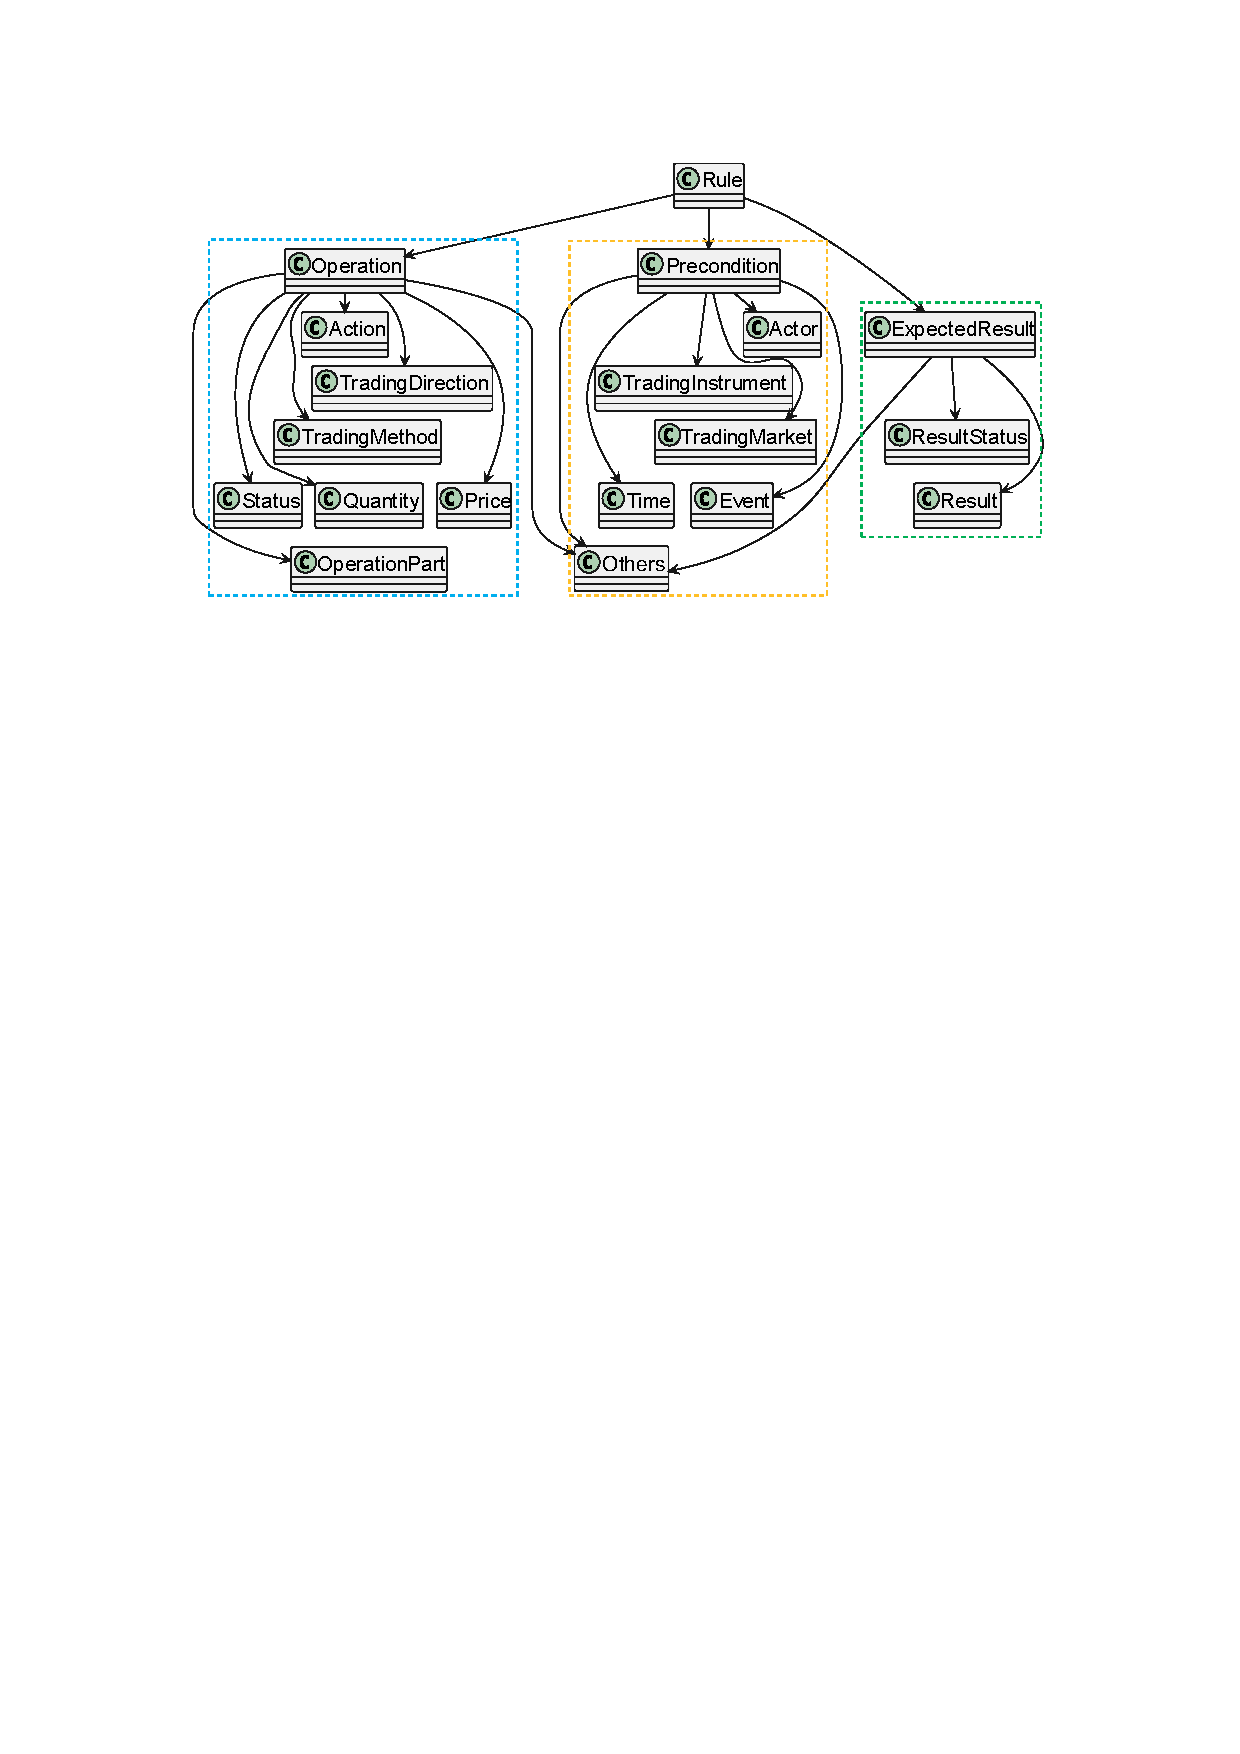
\includegraphics[width=0.7\linewidth]{fig/metamodel_real.pdf}
    \caption{Meta-model for the financial domain.}
    \label{fig:metamodel_real}
    \Description{A hierarchical financial-domain meta-model organizes fourteen entities under precondition, operation, and expected-result categories and shows their relations.}
    \vspace{-2mm}
\end{figure}


\noindent
\textbf{Example of Explicated Regulatory Knowledge.}
We illustrate the artifacts using the default three-LLM ensemble. With 10
regulatory documents, 20 tests, and $N=3$, $K=2$, purification produces
$\mathcal{M}_f$: 14 entities organized under \textit{Precondition},
\textit{Operation}, and \textit{Expected Result} (Fig.~\ref{fig:metamodel_real}).
Fine-grained attributes and values are deferred to $\mathcal{R}_f$.

\begin{figure}[!t]
    \centering
    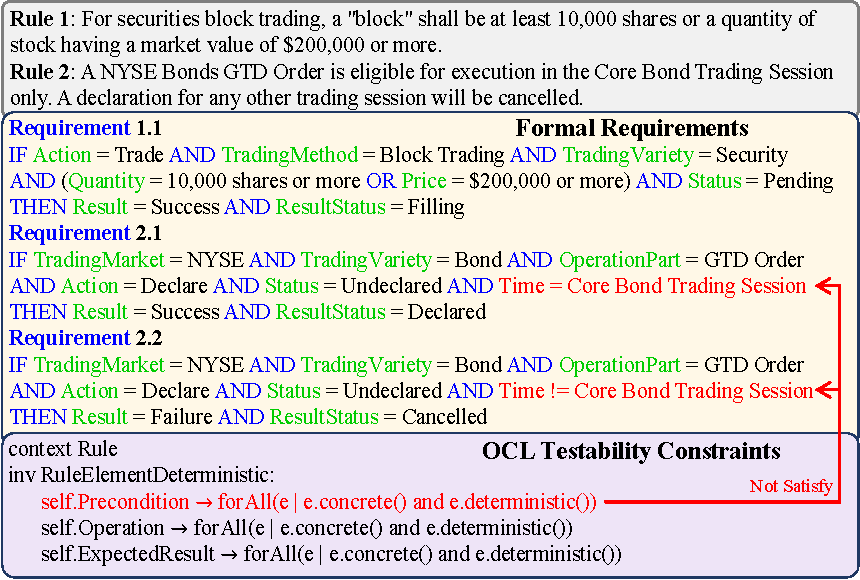
\includegraphics[width=0.7\linewidth]{fig/rule_example.pdf}
    \caption{Two example rules from NYSE~\cite{nyse}, their formal requirements, and their testability decisions.}
    \label{fig:rule_example}
    \Description{Two natural-language NYSE rules are mapped to structured IF-THEN requirements and labeled as testable or untestable according to the five testability dimensions.}
\end{figure}

Each LLM maps $\mathcal{M}_f$ to symbols, a typed data dictionary, and a BNF
syntax~\cite{backus1960report}; aggregation forms $\mathcal{R}_f$ from their
union. Fig.~\ref{fig:rule_example} illustrates its \textit{IF-THEN}
requirements, composed of \textit{KEY-OP-VALUE} expressions joined by
\textit{AND} or \textit{OR}.



Using $\mathcal{R}_f$, the LLMs specify OCL-style constraints~\cite{ocl2014object}
whose union forms $\mathcal{T}_f$. The notation structures LLM assessment but
is not executable OCL. Its five dimensions are structural completeness,
element determinism, action executability, result observability, and rule
non-conflict.
% \begin{enumerate}[leftmargin=*,align=left, itemsep=0pt, parsep=0pt, nosep]
%     \item \textbf{Structural Completeness}, ensuring that the precondition, operation, and expected result are present and not empty.
%     \item \textbf{Element Determinism}, requiring that \textit{KEY} and \textit{VALUE} are deterministic, specific, and free from ambiguity.
%     \item \textbf{Action Executability}, ensuring that operations correspond to concrete actions performable within the system.
%     \item \textbf{Result Observability}, ensuring that expected results are defined and can be objectively measured or verified.
%     \item \textbf{Rule Non-Conflict}, guaranteeing that rules are logically consistent and do not introduce contradictions.
% \end{enumerate}

For example, \textit{Requirement 1.1} in Fig.~\ref{fig:rule_example} satisfies all constraints and is therefore testable, whereas \textit{Requirements 2.1} and \textit{2.2} are deemed untestable because of the non-deterministic expression ``core bond trading session'', which must be concretized as a specific time range (e.g., 9:00--11:30).












\subsection{Phase II: Requirements Formalization and Test Generation}
\label{sec:test_gen}


Phase~II uses knowledge-injected prompting to formalize rules, refine
testability, compose scenarios, and generate implementation-independent tests.


\noindent
\textbf{Knowledge-Injected Prompt Generation.}
In \textit{Step} \ding{175}, two prompts inject the knowledge:

\begin{enumerate}[leftmargin=*,align=left, itemsep=0pt, parsep=0pt, nosep]
    \item $P_\mathcal{R}$ combines $\mathcal{R}$'s schema with task
    decomposition, CoT, and self-critique.
    \item $P_\mathcal{T}$ evaluates each requirement against $\mathcal{T}$ and
    triggers refinement for violations.
\end{enumerate}
$\mathcal{M}$ is not injected directly because it is encoded in $\mathcal{R}$.


\noindent
\textbf{Formal Requirements Generation.}
In \textit{Step} \ding{176}, $P_\mathcal{R}$ adds two workflow annotations:
\textit{Status}, the required pre-operation state, and \textit{ResultStatus},
the expected post-operation state. These annotations define the state boundary
of a requirement and connect otherwise independent requirements into structured
business scenarios when one requirement's post-state satisfies another's
pre-state. They are used only for scenario construction and semantic checking,
not as additional regulatory predicates, and their values must be supported by
the rule or document context.

Our Generate-Verify-Refine loop compiles $\mathcal{R}$'s structured view into
an Xtext syntax validator~\cite{eysholdt2010xtext}. GPT-6-Astra~\cite{gpt}
performs semantic checks: each key must exist in the dictionary, its operator
must be type-compatible, its value must be supported by cited source evidence,
and its state annotations must agree with the operation and outcome. The
checkers return localized diagnostics; refinement changes only flagged
fragments. After three failed repairs, fully automated \ourtool\ discards the
requirement, whereas the HITL variant routes it to expert review. Generated
validators are included in the replication package.




\noindent
\textbf{Testability Determination \& Refinement.}
In \textit{Step} \ding{177}, $P_\mathcal{T}$ uses LLMs to assess each
requirement against every OCL-style predicate by considering the source rule,
document context, structured elements, and logical relationships. The notation
makes each context, predicate, and invariant formally explicit, but predicates
such as determinism and observability require semantic judgment. They are
therefore evaluated by an LLM rather than executed by an OCL engine.

Violations trigger targeted completion or concretization, and the
refined requirement is checked again against $\mathcal{T}$. Every added element
or value must be traceable to the source rule or document context; otherwise,
the requirement remains flagged. Requirements that remain ambiguous, lack
sufficient context, or are inherently untestable are discarded by fully
automated \ourtool\ and routed to expert review only in the HITL variant.





\noindent
\textbf{Scenario \& Test Case Generation.}
In \textit{Step} \ding{178}, testable formal requirements are transformed into
test cases. A requirement precedes another when they concern the same business
object and every canonicalized \textit{ResultStatus} field equals or falls
within the latter's \textit{Status} constraint. Undecidable pairs are not
linked. Chaining these dependencies yields scenario flows; requirements
without state annotations yield only single-rule tests.

Test cases are then generated in two steps. First, Equivalence Partitioning and
Boundary Value Analysis~\cite{graham2006foundations} produce candidate test data
for each constraint. Numerical constraints yield representative valid,
invalid, and boundary values. Finite non-numerical domains are enumerated,
whereas open fields use a satisfying $X$ and a non-satisfying $\neg X$. Second,
these data are assigned to the expression tree encoded by the formal
requirement. The expected validity is the truth value of the complete
expression, evaluated recursively under its operators: conjunction requires
all operands, disjunction requires at least one operand, and implication
$A\Rightarrow B$ is violated only when $A$ is true and $B$ is false. An
assignment with a false antecedent is therefore an antecedent-inactive valid
case, not a violation.

\begin{table}[!t]
    \setlength{\tabcolsep}{8pt}
    \captionsetup{skip=2pt}
    \caption{Selected test cases for \textit{Rule 1} in Fig.~\ref{fig:rule_example}. \textit{Case 4} succeeds because another rule governs that scenario.}
    \label{tab:testcase_example}
    \centering
    \resizebox{\linewidth}{!}{
    \begin{tabular}{|cccccccc|}
    \hline
        \textbf{Test Case} & \textbf{Trading Market} & \textbf{
        Trading Variety} & \textbf{Trading Method} & \textbf{Action} & \textbf{Quantity} & \textbf{Price} & \textbf{Result} \\
        \hline
        \textbf{1} & NYSE & Security & Block Trading & Trade & 50K SH & \$500K & Success \\
        \textbf{2} & NYSE & Security & Block Trading & Trade & 10K SH & \$500K & Success \\
        \textbf{3} & NYSE & Security & Block Trading & Trade & 9K SH & \$100K & Failure \\
        \textbf{4} & NYSE & Security & Auction Trading & Trade & 50K SH & \$500K & Success \\
        \hline
    \end{tabular}
    }
\end{table}


Candidate assignments include active and inactive antecedents. Before pairwise
generation, representative sampling retains one canonical value per
equivalence class; Pairwise Coverage then ensures that each retained value pair
appears in at least one case~\cite{kuhn2004software,myers2004art}. Expected
outcomes and post-states follow the full-expression evaluation
(Table~\ref{tab:testcase_example}). The outputs are compliance test cases with
inputs, actions, expected outcomes, and state transitions.

Each emitted case retains the originating requirement and rule identifiers,
selected equivalence class or boundary value, and full-expression outcome.
This metadata supports audits from each expected result to its source clause
and distinguishes rule-derived values from knowledge-assisted structure; it is
not used as an additional regulatory predicate.


%Pairwise Coverage \cite{kuhn2008automated} is applied, yielding a compact yet comprehensive set of test cases.
%, as exemplified in Table~\ref{tab:testcase_example}.
% We integrate the testable structured requirements into a model-based test case generation workflow. Based on a survey of related work, we adopt LLM4Fin~\cite{xue2024llm4fin}, which is most compatible with our requirement representation. The adapted workflow consists of two stages: Test Scenario Construction, and Test Case Generation.

% Test scenarios are constructed by identifying inter-rule dependencies. Behavioral elements such as \textit{Action} and \textit{Status} are mapped to predefined activity diagrams and state machines, linking individual requirements into end-to-end business flows.

% For each scenario, concrete test cases are derived using diverse test strategies such as Equivalence Partitioning and Boundary Value Analysis \cite{graham2006foundations}. Numerical inputs yield representative positive, negative, and boundary values, while finite non-numerical inputs are exhaustively enumerated. To mitigate combinatorial explosion, Pairwise Coverage \cite{kuhn2008automated} is applied to produce a compact yet comprehensive set of test cases, with an example shown in Table~\ref{tab:testcase_example}.

% Finally, test cases are generated from testable requirements. We apply test strategies such as equivalence class and boundary value analysis \cite{graham2006foundations} to the constraints. Specifically, for numerical constraints, several representative positive, negative, and boundary values are generated. For non-numerical constraints, all values will be enumerated if the value domain is finite; otherwise, only the value itself is used.
% To avoid a combinatorial explosion when multiple constraints interact, we do not perform a full Cartesian product \cite{kuhn2015combinatorial}. Instead, we apply lightweight strategies such as pairwise coverage \cite{kuhn2008automated} and representative sampling. This results in a compact yet comprehensive set of test cases that covers positive, negative, and boundary cases. Table \ref{tab:testcase_example} shows part of the test cases generated for \textit{Rule 1} in Figure \ref{fig:rule_example}.


\section{Experimental Evaluation}
\label{sec:experiment}

We organize the evaluation around five research questions that progress from
end-to-end utility to component attribution, step-level behavior, model
sensitivity, and cross-domain workflow re-instantiation:
\begin{enumerate}[leftmargin=*,align=left, itemsep=0pt, parsep=0pt, nosep]
    \item[\textbf{RQ1:}] How does \ourtool\ compare with expert and automated baselines in test-case fidelity, scenario adequacy, efficiency, and monetary cost?
    \item[\textbf{RQ2:}] How much do the explicated knowledge artifacts and optional construction corpus contribute to test quality, and how does artifact-specific consolidation affect downstream performance?
    \item[\textbf{RQ3:}] How accurately and efficiently do Requirements Generation and Testability Determination perform?
    \item[\textbf{RQ4:}] How sensitive is \ourtool\ to the choice of the underlying LLM backbone?
    \item[\textbf{RQ5:}] How consistently can the fixed \ourtool\ workflow be re-instantiated for different regulatory document families?
\end{enumerate}

\noindent
\textbf{Common Implementation and Protocol.}
We implement \ourtool\ as a modular Python workflow that generates test cases from
regulations while retaining all intermediate artifacts for traceability. As
shown in Fig.~\ref{fig:framework}, the workflow comprises seven sequential
steps. Candidate and downstream generation use
GPT-6-Astra~\cite{gpt}, Grok-4.7~\cite{grok}, and
Gemini-3.8-Flash~\cite{gemini}; GPT-6-Astra also performs semantic alignment
and semantic checking. The knowledge-explication steps
(\ding{172}--\ding{174}) use stochastic decoding
(\texttt{temperature}=0.8, \texttt{top\_p}=0.9) to obtain diverse candidates,
whereas downstream generation (\ding{175}--\ding{177}) uses greedy decoding
(\texttt{temperature}=0, \texttt{do\_sample}=false) for consistency. Unless an
experiment varies these settings, \ourtool\ uses $N=3$ and strict-majority threshold
$K=2$. These defaults are fixed before any evaluation: $N=3$ follows from the
three independent LLM backends, and $K=2$ is the corresponding strict-majority
rule rather than a value selected from downstream scores. Prompt and decoding
choices are finalized using only the construction corpus. The evaluation
datasets are never used for hyperparameter selection.

The citations record provider documentation and access dates for the exact
model identifiers used. Their immutable weights are not exposed; unlisted
request fields use provider defaults, and no portable random seed is available
across the three APIs.

For each domain, the construction corpus and the evaluation datasets are
disjoint at the document, rule, and test-case levels, as described in
Section~\ref{sec:know_ext}. One \ourtool\ run has two stages. First, all three
LLMs are required to generate candidate versions of $\mathcal{M}$,
$\mathcal{R}$, and $\mathcal{T}$, which are consolidated into one shared
knowledge bundle and frozen for that run. Second, GPT-6-Astra, Grok-4.7, and
Gemini-3.8-Flash each use the shared bundle to independently generate test
cases. Each backend output is matched and scored separately, yielding three
metric observations. We repeat the complete two-stage run three times,
regenerating the candidate artifacts each time, and report the mean of the
resulting nine observations per dataset.

An E2E run likewise yields one independently scored output per backend.
Single-backend baselines are averaged over three runs.
Preconstructed gold formal requirements, testability labels, partner
ground-truth test cases, and scenario labels are used only by the offline
evaluator. No best-run output is selected or
substituted. Prompts, request parameters, model identifiers, timestamps, and
evaluator inputs are logged with each run. Timing measurements include
orchestration and API latency and are collected under the same workflow
conditions. Experiment~IV reports fidelity against reference test cases only; it does not
compare hardware-dependent open-weight inference time.

All financial-domain experts were senior testing engineers with 3--5 years of
relevant experience. Independent double annotation of gold items, artifacts,
and equivalence decisions achieved over 90\% initial item-level agreement;
remaining disagreements were resolved by discussion against the source
regulations.

\subsection{Experiment I: Overall Performance}
\label{sec:exp1}

Experiment~I addresses RQ1 in the financial domain. It compares fully
automated methods, an expert baseline, and an optional assisted configuration
so that automation and human intervention are not conflated.

\noindent
\textbf{Competitors.}
We compare \ourtool\ with five baseline categories: (i) \textit{Domain
Experts}, three senior testing engineers with 3--5 years of financial-domain
experience; (ii) \textit{E2E LLMs}, in which the three LLMs used by \ourtool\
directly generate tests from regulatory documents with strong prompting;
(iii) ACC-Fra, our financial-domain adaptation of an ontology-guided automated
compliance-checking architecture originally evaluated on BIM~\cite{chen2024automated}; (iv) the multi-stage
LLM-based MSG-Spec~\cite{milchevski2025multi}; and (v) the hybrid LLM4Fin
framework~\cite{xue2024llm4fin}. We additionally report
\textit{\ourtool\ + HITL}, in which two experts who are distinct from the
expert-baseline participants correct formal requirements and testability
decisions before test generation. The expert baseline and \ourtool\ + HITL are
therefore human and assisted settings, respectively, rather than fully
automated competitors.

We distinguish two comparison roles. The controlled comparison is E2E LLMs:
each of the same three backends used by \ourtool\ directly generates tests,
and both methods use the same evaluation documents, output fields, frozen
matcher, and three-run protocol. Experiment~IV additionally pairs \ourtool\
and E2E generation separately for each of 11 open-weight models, controlling
the backbone explicitly. ACC-Fra, MSG-Spec, and LLM4Fin are system-level
comparisons reimplemented from their published descriptions or run with
default configurations where available. Because their backbones and workflows
differ, these rows compare complete systems rather than isolating the causal
effect of \ourtool. We do not force
equal token counts, which would truncate methods with different output
structures; instead, Table~\ref{tab:exp1_token} reports observed tokens and
cost so quality and resource use can be interpreted jointly.

\noindent
\textbf{Datasets.} 
Due to limited public benchmarks, we construct six financial datasets from
official exchange regulations, each paired with an anonymized partner-maintained
industrial test cases---the sole ground truth for all automated and expert
baselines. They span auction, options, and bond rules across jurisdictions and
languages and vary in size and complexity. None of these held-out datasets
(Table~\ref{tab:exp1_dataset}) constructs $\mathcal{M}$, $\mathcal{R}$, or
$\mathcal{T}$.

\begin{table*}[!t]
    \setlength{\tabcolsep}{2pt}
    \caption{Details of the six financial datasets used in Experiment I. ``\#'' denotes the number of Rules, Nested Rules (Nest.), Dependent Rule Pairs (Dep.), Requirements (Req.), Fine-Grained Constraints (Cons.), and Test Cases (TC).}
    \label{tab:exp1_dataset}
    \centering
    \resizebox{\linewidth}{!}{
    \begin{tabular}{|c|l|c|c|c|c|c|c|}
    \hline
        \textbf{Dataset} & \textbf{Document} & \textbf{\# Rule} & \textbf{\# Nest.} & \textbf{\# Dep.} & \textbf{\# Req.} & \textbf{\# Cons.} & \textbf{\# TC} \\
        \hline
        \textbf{1} & New York Stock Exchange Auction Market Bids and Offers Rules \cite{dataset1} & 142 & \textbf{77} & \textbf{58} & 114 & 344 & 927 \\
        \textbf{2} & The Nasdaq Stock Market Options Trading Rules \cite{dataset2} & 289 & \textbf{48} & 35 & \textbf{276} & \textbf{706} & 1465 \\
        \textbf{3} & Hong Kong Stock Exchange Trading Rules \cite{dataset3} & 129 & 21 & 19 & \textbf{292} & \textbf{928} & \textbf{2128} \\
        \textbf{4} & Shanghai Stock Exchange Trading Rules \cite{dataset4} & 212 & 13 & \textbf{48} & 195 & 244 & 682 \\
        \textbf{5} & Shenzhen Stock Exchange Bond Trading Rules \cite{dataset5} & 190 & 16 & 32 & 167 & 571 & 1389 \\
        \textbf{6} & Tokyo Stock Exchange Buying and Selling Rules \cite{dataset6} & 104 & \textbf{41} & 28 & 198 & 382 & 1020 \\
        \hline
    \end{tabular}
    }
\end{table*}

\noindent
\textbf{Test-Case Fidelity Metrics.}
We match generated test cases to partner-maintained reference cases using a
frozen one-to-one matcher. It compares only behavioral fields in
the shared industrial schema and ignores provenance, including source-rule
identifiers and evidence; source annotations need not agree. Behavioral field
sets must be identical. Numerical values match within the same expert-defined
valid, invalid, or boundary equivalence class. Non-numerical values use the
multilingual
\texttt{paraphrase-multilingual-mpnet-base-v2} SentenceTransformer
model~\cite{reimers2019sentence}. Experts selected and froze 0.85 before
evaluation because lower thresholds admitted semantically distinct pairs,
whereas higher thresholds rejected valid paraphrases.
Polarity, negation, and comparison operators must agree, and every field must
match. Maximum-cardinality bipartite matching prevents duplicate counting.
Given matched pairs $m$, generated cases $n_g$, and
reference cases $n_r$, we compute $P=m/n_g$, $R=m/n_r$, and
$F1=2PR/(P+R)$.

We also report \textit{Business Scenario Coverage (BSC)} as scenario
adequacy~\cite{xue2024llm4fin}, defined as $\mathit{BSC}=p_t/p_a$, where $p_t$
is the number of covered reference business scenarios and $p_a$ is the total
number of reference business scenarios. A reference scenario is covered only
when every constituent step has a test case matched by the same rules above
and the generated \textit{Status}/\textit{ResultStatus} transitions preserve
the reference dependency order. Higher BSC indicates broader coverage of
regulatory requirements and scenarios under rule changes.

Efficiency is workflow elapsed
time, decomposed into knowledge explication, generation, and applicable expert
review. Because hardware and review requirements differ, totals are descriptive
rather than quality-normalized speedups; human effort is reported separately
in person-hours and is not added to wall-clock time. Prompt and completion
tokens come from per-request provider usage records, and monetary cost is the
corresponding provider-billed API charge. Local compute and labor are not
converted into dollars.

\noindent
\textbf{Experimental Procedure.}
Three domain experts independently authored test cases for each dataset using
the partner workflow. Their cases are baselines, not ground truth, and are
scored against the same partner cases as automated methods. Each expert created
requirement-level templates and equivalence partitions, then instantiated cases
in batches. Active-work logs cover interpretation, condition and template
design, expected outcomes, and review while excluding breaks. They record a
mean 42.56 person-hours for reference-sized test cases, or 20.13 seconds per
instantiated case across 7,611 cases. Scores and effort are averaged across the
three experts.

The E2E prompts combine four performance-oriented techniques: (i) task-specific
instructions; (ii) few-shot examples of high-quality rules and test cases;
(iii) CoT prompting for element extraction, testability determination, and test
generation; and (iv) self-reflection for output refinement.

The implementations of ACC-Fra and MSG-Spec are not publicly available, so we
reimplemented them from their original papers. For ACC-Fra, we retain the published
ontology-guided extraction and checking stages but adapt their inputs and
outputs to financial regulations and the shared industrial test-case schema.
The open-source LLM4Fin runs with its default configuration.
For \ourtool, the three LLMs jointly explicate knowledge through consensus;
each LLM then generates test cases independently.

All LLM-based methods use the same evaluation documents and are run three
times under the same output schema and evaluation protocol. Thus, \ourtool\ and
E2E cells average nine outputs (three backends $\times$ three runs);
single-backend baselines average three runs and expert cells average three
individuals.

The Average row is the macro-average across datasets, and the
final row is the sample variance of the six dataset means. In
Table~\ref{tab:exp1}, light and dark red denote scores of 60--90\% and above
90\%, respectively, and bold marks the best result per metric. We use paired
exact Wilcoxon tests over the six datasets, Holm-correct the five comparisons
per metric, and report matched-pairs rank-biserial effect sizes. We also conduct
two one-sided tests (TOST) of practical equivalence between fully automated
\ourtool\ and the experts with a predefined $\pm5$-point margin.



\begin{table*}[!t]
    \setlength{\tabcolsep}{2pt}
    \centering
    \caption{Test-case fidelity (precision, recall, and F1) and business-scenario coverage (BSC) on the six financial datasets (\%).}
    \label{tab:exp1}

    % ====== 颜色定义区 ======
    \colorlet{ColorLight}{red!8}  % 浅红色：用于 60 到 90 之间的值
    \colorlet{ColorDark}{red!25}  % 深红色：用于 90 及以上的值
    % ========================

    % 自动判断宏（普通数值）
    \newcommand{\cc}[1]{%
        \ifdim #1 pt < 60 pt\relax
            #1%
        \else
            \ifdim #1 pt < 90 pt\relax
                \cellcolor{ColorLight}#1%
            \else
                \cellcolor{ColorDark}#1%
            \fi
        \fi
    }

    % 自动判断宏（加粗数值）
    \newcommand{\ccb}[1]{%
        \ifdim #1 pt < 60 pt\relax
            \textbf{#1}%
        \else
            \ifdim #1 pt < 90 pt\relax
                \cellcolor{ColorLight}\textbf{#1}%
            \else
                \cellcolor{ColorDark}\textbf{#1}%
            \fi
        \fi
    }

    \resizebox{\linewidth}{!}{
    \begin{tabular}{@{} c *{28}{c} @{}}
        \toprule
        \multirow{2}{*}{\textbf{Datasets}} &
        \multicolumn{4}{c}{\textbf{Domain Experts}} &
        \multicolumn{4}{c}{\textbf{E2E LLMs}} &
        \multicolumn{4}{c}{\textbf{ACC-Fra}} &
        \multicolumn{4}{c}{\textbf{MSG-Spec}} &
        \multicolumn{4}{c}{\textbf{LLM4Fin}} &
        \multicolumn{4}{c}{\textbf{\ourtool}} &
        \multicolumn{4}{c}{\textbf{\ourtool\ + HITL}} \\
        \cmidrule(lr){2-5} \cmidrule(lr){6-9} \cmidrule(lr){10-13} \cmidrule(lr){14-17} \cmidrule(lr){18-21} \cmidrule(lr){22-25} \cmidrule(l){26-29}
        & Pre. & Rec. & F1 & BSC & Pre. & Rec. & F1 & BSC & Pre. & Rec. & F1 & BSC & Pre. & Rec. & F1 & BSC & Pre. & Rec. & F1 & BSC & Pre. & Rec. & F1 & BSC & Pre. & Rec. & F1 & BSC \\
        \midrule
        \textbf{1} & \cc{84.6} & \cc{95.2} & \cc{89.6} & \cc{85.1} & \cc{6.8} & \cc{45.3} & \cc{11.8} & \cc{11.2} & \cc{33} & \cc{47.6} & \cc{38.9} & \cc{37} & \cc{42.7} & \cc{99.4} & \cc{59.7} & \cc{56.8} & \cc{77.1} & \cc{72.8} & \cc{74.9} & \cc{71.2} & \cc{93.9} & \cc{96.9} & \cc{95.3} & \cc{90.6} & \ccb{92.8} & \ccb{100} & \ccb{96.2} & \ccb{91.4} \\
        \textbf{2} & \cc{85.8} & \cc{97.1} & \cc{91.1} & \cc{86.5} & \cc{6.9} & \cc{38.4} & \cc{11.7} & \cc{11.1} & \cc{47.9} & \cc{40.6} & \cc{43.9} & \cc{41.7} & \cc{38} & \cc{94.7} & \cc{54.2} & \cc{51.5} & \cc{51.9} & \cc{73.4} & \cc{60.8} & \cc{57.8} & \cc{82.6} & \cc{87} & \cc{84.7} & \cc{80.5} & \ccb{90.3} & \ccb{99.9} & \ccb{94.9} & \ccb{90.1} \\
        \textbf{3} & \cc{94} & \ccb{100} & \cc{96.9} & \ccb{92.1} & \cc{13.5} & \cc{22.2} & \cc{16.8} & \cc{16} & \cc{43.1} & \cc{53.3} & \cc{47.7} & \cc{37.3} & \cc{49.4} & \cc{99.4} & \cc{66} & \cc{62.7} & \cc{74.2} & \cc{77.1} & \cc{75.6} & \cc{71.8} & \ccb{94.9} & \cc{95.3} & \cc{95} & \cc{90.2} & \cc{94.4} & \cc{100} & \ccb{97.1} & \cc{92.3} \\
        \textbf{4} & \ccb{90.2} & \cc{97.3} & \cc{93.6} & \cc{88.9} & \cc{30.5} & \cc{37.7} & \cc{33.7} & \cc{32} & \cc{51.7} & \cc{46.6} & \cc{49} & \cc{46.6} & \cc{54.8} & \cc{95.4} & \cc{69.6} & \cc{66.1} & \cc{59.9} & \cc{82.3} & \cc{69.3} & \cc{65.8} & \cc{81.8} & \ccb{94.8} & \cc{87.8} & \cc{83.4} & \cc{90.5} & \cc{100} & \ccb{95} & \ccb{90.2} \\
        \textbf{5} & \ccb{93.4} & \cc{100} & \cc{96.6} & \cc{91.8} & \cc{31.5} & \cc{35.3} & \cc{33.3} & \cc{31.6} & \cc{100} & \cc{36.7} & \cc{53.7} & \cc{51} & \cc{56.7} & \cc{98.4} & \cc{72} & \cc{68.4} & \cc{61} & \cc{88.1} & \cc{72.1} & \cc{68.5} & \cc{99.3} & \cc{93.6} & \cc{96.4} & \cc{91.6} & \cc{94.5} & \ccb{99.9} & \ccb{97.1} & \ccb{92.2} \\
        \textbf{6} & \cc{91.8} & \cc{100} & \cc{95.7} & \cc{90.9} & \cc{17.9} & \cc{38.6} & \cc{24.4} & \cc{23.2} & \cc{22.7} & \cc{96.3} & \cc{36.7} & \cc{34.9} & \cc{37.1} & \cc{98.4} & \cc{53.9} & \cc{51.2} & \cc{81.3} & \cc{42.4} & \cc{55.7} & \cc{52.9} & \cc{91.1} & \cc{90.8} & \cc{90.9} & \cc{86.4} & \ccb{93.9} & \ccb{100} & \ccb{96.8} & \ccb{92} \\
        \midrule
        \textbf{Average} & \cc{90} & \cc{98.3} & \cc{93.9} & \cc{89.2} & \cc{17.8} & \cc{36.3} & \cc{21.9} & \cc{20.9} & \cc{49.7} & \cc{53.5} & \cc{45.0} & \cc{41.4} & \cc{46.5} & \cc{97.6} & \cc{62.6} & \cc{59.5} & \cc{67.6} & \cc{72.7} & \cc{68.1} & \cc{64.7} & \cc{90.6} & \cc{93} & \cc{91.7} & \cc{87.1} & \textbf{\cc{92.7}} & \textbf{\cc{99.9}} & \textbf{\cc{96.2}} & \textbf{\cc{91.4}} \\
        \textbf{Cross-dataset Var.} & 15.5 & 4.1 & 9.2 & 8.4 & 121.5 & 58.5 & 101.5 & 91.4 & 717.8 & 472.6 & 41.3 & 39.5 & 71.3 & 4.2 & 60.7 & 54.6 & 134.2 & 253.5 & 65.4 & 59 & 49.4 & 13 & 22.2 & 20 & 3.6 & 0 & 1 & 1 \\
        \bottomrule
    \end{tabular}
    }
\end{table*}

\noindent
\textbf{Experimental Results.}
Table~\ref{tab:exp1} reports test-case fidelity and scenario adequacy.
Among fully automated methods, \ourtool\ has the highest F1 and BSC on every
dataset, with macro-averages of 91.7\% and 87.1\%, respectively. Relative to
the strongest automated baseline, LLM4Fin, the observed differences are 23.6
F1 points and 22.4 BSC points; relative to direct E2E generation, they are 69.8
and 66.2 points. The latter is the backbone-matched workflow comparison; the
former is a system-level comparison. \ourtool's F1 cross-dataset variance (22.2) is also
below that of every automated baseline (41.3--101.5), indicating more
consistent fidelity to the reference cases
across the six documents. The causal role of explicit artifacts, rather than
the end-to-end comparison alone, is examined in Experiment~II.

The five planned comparisons comprise four automated baselines and the expert
baseline. Against each automated baseline, every dataset-level difference
favors \ourtool\ ($r_{\mathrm{rb}}=1$; exact $p=0.031$); Holm correction across
all five gives $p_{\mathrm{H}}=0.156$. Thus, none establishes corrected
superiority at $\alpha=0.05$. The expert comparison is not uniformly
directional: \ourtool\ is 2.2 F1 and 2.1 BSC points below the expert mean. TOST
also does not establish equivalence within $\pm5$ points: the F1 90\% CI is
$[-6.0,+1.5]$ ($p_{\mathrm{TOST}}=0.099$), and the BSC CI is
$[-5.7,+1.5]$ ($p_{\mathrm{TOST}}=0.081$).

Correcting the two intermediate artifacts in \ourtool\ + HITL yields
92.7\%/99.9\%/96.2\%/91.4\% in P/R/F1/BSC. These means exceed the expert
baseline by 2.3 on F1 and 2.2 on BSC. The variant's lower cross-dataset
variance indicates that upstream correction benefits all six datasets.
This assisted result is descriptive and is not included in the five-comparison
inferential family.


\begin{figure}[!t]
    \centering
    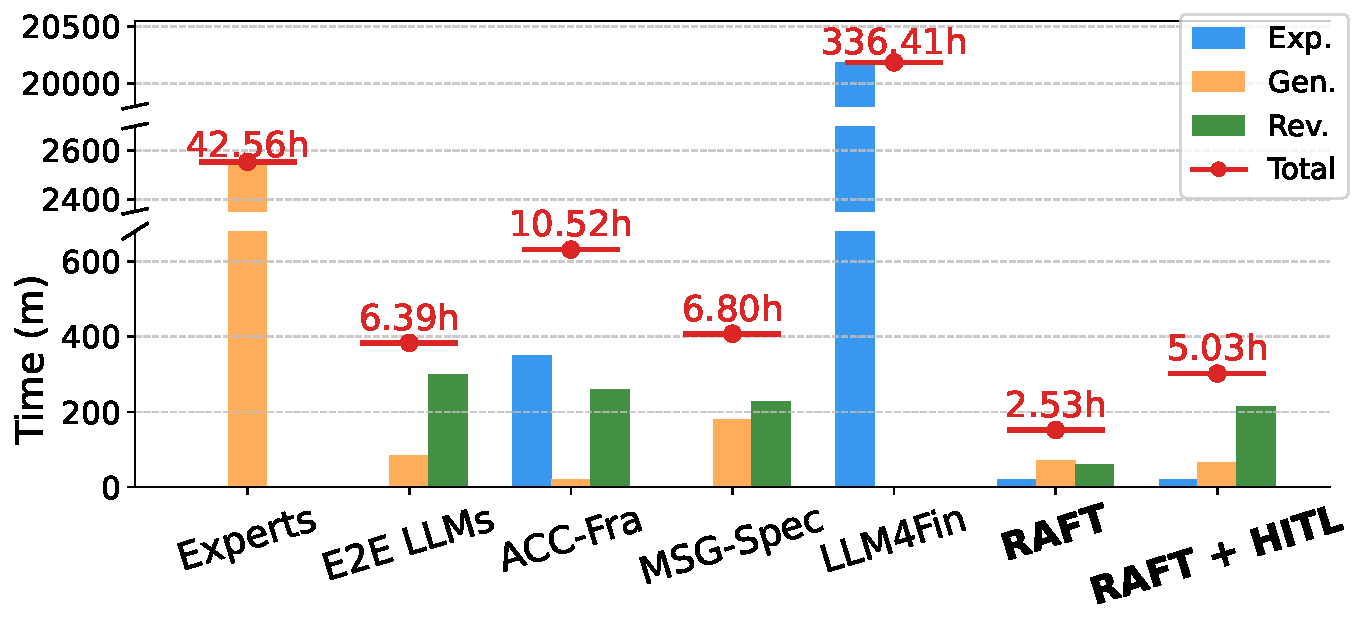
\includegraphics[width=0.60\linewidth]{fig/exp1_time.pdf}
    \caption{Elapsed workflow time across the six financial datasets. Exp., Gen., and Rev.\ denote knowledge explication, test generation, and review or repair.}
    \label{fig:exp1_time}
    \Description{A broken-axis bar chart compares end-to-end time for experts, four baselines, RAFT, and RAFT plus HITL. The measured expert workflow takes 42.56 person-hours; RAFT and its HITL variant take 2.53 and 5.03 hours of elapsed time, respectively. The HITL review requires 7.16 person-hours.}
\end{figure}








\begin{table}[!t]
    \setlength{\tabcolsep}{35pt}
    \caption{Observed per-dataset token usage and provider-billed API cost on the six financial datasets.}
    \label{tab:exp1_token}
    \centering
    \resizebox{\linewidth}{!}{
    \begin{tabular}{|c|c|c|c|}
    \hline
    \textbf{Method} & \textbf{Prompt Tokens} & \textbf{Completion Tokens} & \textbf{API Cost (\$)} \\
    \hline
    \textbf{E2E LLMs} & 115,842 & 1,328,617 & 26.947 \\
    \textbf{MSG-Spec} & 342,517 & 1,685,236 & 35.018 \\
    \textbf{LLM4Fin} & 227,341 & 114,812 & -- \\
    \textbf{\ourtool} & 1,047,286 & 352,043 & 11.463 \\
    \hline
    \end{tabular}
    }
    
\end{table}


Fig.~\ref{fig:exp1_time} reports the elapsed time of each implemented
workflow. Fully automated \ourtool\ completes all six datasets in 2.53 hours.
\ourtool\ + HITL takes 5.03 wall-clock hours: 1.45 hours for its automated stages
and 3.58 hours for concurrent expert review. The review logs record a mean of
10.37 seconds for each of the 1,242 requirement--testability decision pairs for
each expert. Two experts therefore contribute 7.16
person-hours; person-hours are reported separately rather than added to elapsed
time. The measured single-expert workflow requires 42.56 person-hours under the
logged batch-template workflow. We report absolute values, not speedup factors,
because the automated workflows have different execution and review
requirements.





As shown in Table~\ref{tab:exp1_token}, the G-V-R and OCL Cons.\ stages in
Table~\ref{tab:exp3_} contribute 107,734 prompt tokens and 320,059 completion
tokens per dataset. The totals add amortized domain-level knowledge explication
and repeated knowledge injection. Per-request usage and billing records retain
the model identifier, prompt tokens, completion tokens, and charged amount for
GPT-6-Astra, Grok-4.7, and Gemini-3.8-Flash. Aggregating these records by method
and reporting the mean across the six datasets gives 1,047,286 prompt tokens,
352,043 completion tokens, and an actual API charge of \$11.463 per dataset for
\ourtool. The corresponding actual charges for E2E LLMs and MSG-Spec are
\$26.947 and \$35.018,
primarily because \ourtool\ produces substantially fewer completion tokens.
LLM4Fin has no API charge because it is deployed locally; the table therefore
should not be read as a total-cost comparison that includes hardware. All API
figures are observed provider charges; local compute and labor are excluded.


\noindent\textbf{Answer to RQ1.}
\ourtool\ has the highest descriptive result among automated methods
(91.7\% F1, 87.1\% BSC) at an actual API cost of \$11.463 per dataset. The differences favor
\ourtool\ on all six datasets, but no superiority comparison remains
significant after Holm correction; HITL reaches 96.2\% F1 without establishing
equivalence to experts.






\subsection{Experiment II: Ablation Study}
\label{sec:exp2}

\noindent
\textbf{Experimental Design.}
Experiment~II addresses RQ2 through four controlled analyses.
First, an \emph{artifact ablation} compares full \ourtool\
($\mathcal{M}{+}\mathcal{R}{+}\mathcal{T}$) with
(i) $\mathcal{M}{+}\mathcal{R}$, which omits testability constraints and
generates from all formal requirements; (ii) $\mathcal{T}$, which omits the
meta-model and requirements representation and applies testability guidance
directly to regulatory rules; and (iii) \textit{No Knowledge}, which uses no
explicit artifacts.
Here, \textit{No Knowledge} means ``no explicit artifacts''; it does not
remove parametric knowledge from the LLM. The E2E baseline in Experiment~I
instead removes the staged formalization workflow and generates tests directly.

The ablation units follow the dependency chain
$\mathcal{M}\rightarrow\mathcal{R}\rightarrow\mathcal{T}$. In particular,
$\mathcal{R}$ defines its symbols, data dictionary, and grammar over the
entities and relations in $\mathcal{M}$, while $\mathcal{M}$ has no direct
downstream interface and becomes operational only through $\mathcal{R}$.
Consequently, an $\mathcal{M}$-only configuration cannot formalize
requirements. Conversely, a frozen $\mathcal{R}$ generated from $\mathcal{M}$
already encodes its entities and structure, so calling it
``$\mathcal{R}$-only'' would not remove the effect of $\mathcal{M}$; regenerating
$\mathcal{R}$ without $\mathcal{M}$ would change the construction process and
allow the LLM to reconstruct an implicit meta-model. The same issue applies to
$\mathcal{R}{+}\mathcal{T}$. We therefore treat
$\mathcal{M}{+}\mathcal{R}$ as a coupled structural unit and compare only
implemented pipeline configurations. These ablations measure the contribution
of valid knowledge bundles and testability guidance, not independent causal
effects for $\mathcal{M}$ and $\mathcal{R}$.

Second, a \emph{construction-source analysis} tests whether useful meta-level
artifacts can be constructed without external domain documents or historical
tests, and how much the optional corpus improves the resulting workflow.
\ourtool\ w/o Corpus constructs the same three artifacts from the domain/task
description and LLM parametric knowledge. The held-out evaluation regulations
are still supplied in Phase~II as the source of rule-specific semantics.
\textit{Full-Corpus Prompting} supplies the entire construction corpus directly
to the LLM in each generation prompt but does not transform it into explicit
artifacts, while
\ourtool\ w/ Expert Artifacts replaces automatically explicated artifacts with
expert-constructed ones.

Third, a \emph{multi-LLM analysis} contrasts joint use
of GPT-6-Astra, Grok-4.7, and Gemini-3.8-Flash with each backend alone.

Finally, an \emph{end-to-end operator-assignment analysis} compares
all-purification, all-aggregation, the reversed assignment, and \ourtool's
assignment. Each setting restarts Phase~I from the same source inputs and run
seed. After setting-specific consolidation of $\mathcal{M}$, the LLMs
regenerate $\mathcal{R}$ candidates conditioned on that $\mathcal{M}$; after
consolidating $\mathcal{R}$, they likewise regenerate $\mathcal{T}$ candidates.
Phase~II then regenerates the formal requirements and tests. Thus, settings do
not share downstream candidate artifacts whose inputs have changed.

We also vary $N$ and $K$; the $N=2$ result averages all three LLM pairs. The
default operator assignment and $N=3$, $K=2$ are frozen before evaluation; these
variants form a preplanned sensitivity analysis and are not used to choose the
reported default.

Artifact quality is measured against expert-consensus artifacts. Atomic
elements are entities and relations for $\mathcal{M}$; symbols, dictionary
entries, and grammar productions for $\mathcal{R}$; and individual constraints
for $\mathcal{T}$. Two experts independently judge whether normalized elements
are semantically equivalent and reconcile disagreements. These decisions are
used to compute artifact-level Precision and Recall. All four analyses also
report downstream F1 and BSC. The remaining evaluation follows Experiment~I.



\noindent
\textbf{Experimental Results.}
Fig.~\ref{fig:exp2} shows a monotonic loss as guidance is removed. Relative
to full \ourtool, $\mathcal{M}{+}\mathcal{R}$ reduces mean Precision by 33.6\%
and Recall by 19.5\%. The larger Precision loss is consistent with the role of
$\mathcal{T}$: without a testability filter, non-testable rules produce
additional unmatched cases. Retaining only $\mathcal{T}$ causes still larger
relative losses (74.8\% in Precision and 39.6\% in Recall), showing that
testability guidance cannot replace the structural vocabulary and grammar in
$\mathcal{M}$ and $\mathcal{R}$. \textit{No Knowledge} is lowest on every
metric; F1 and BSC follow the same ordering.

\begin{figure*}[!t]
    \centering
    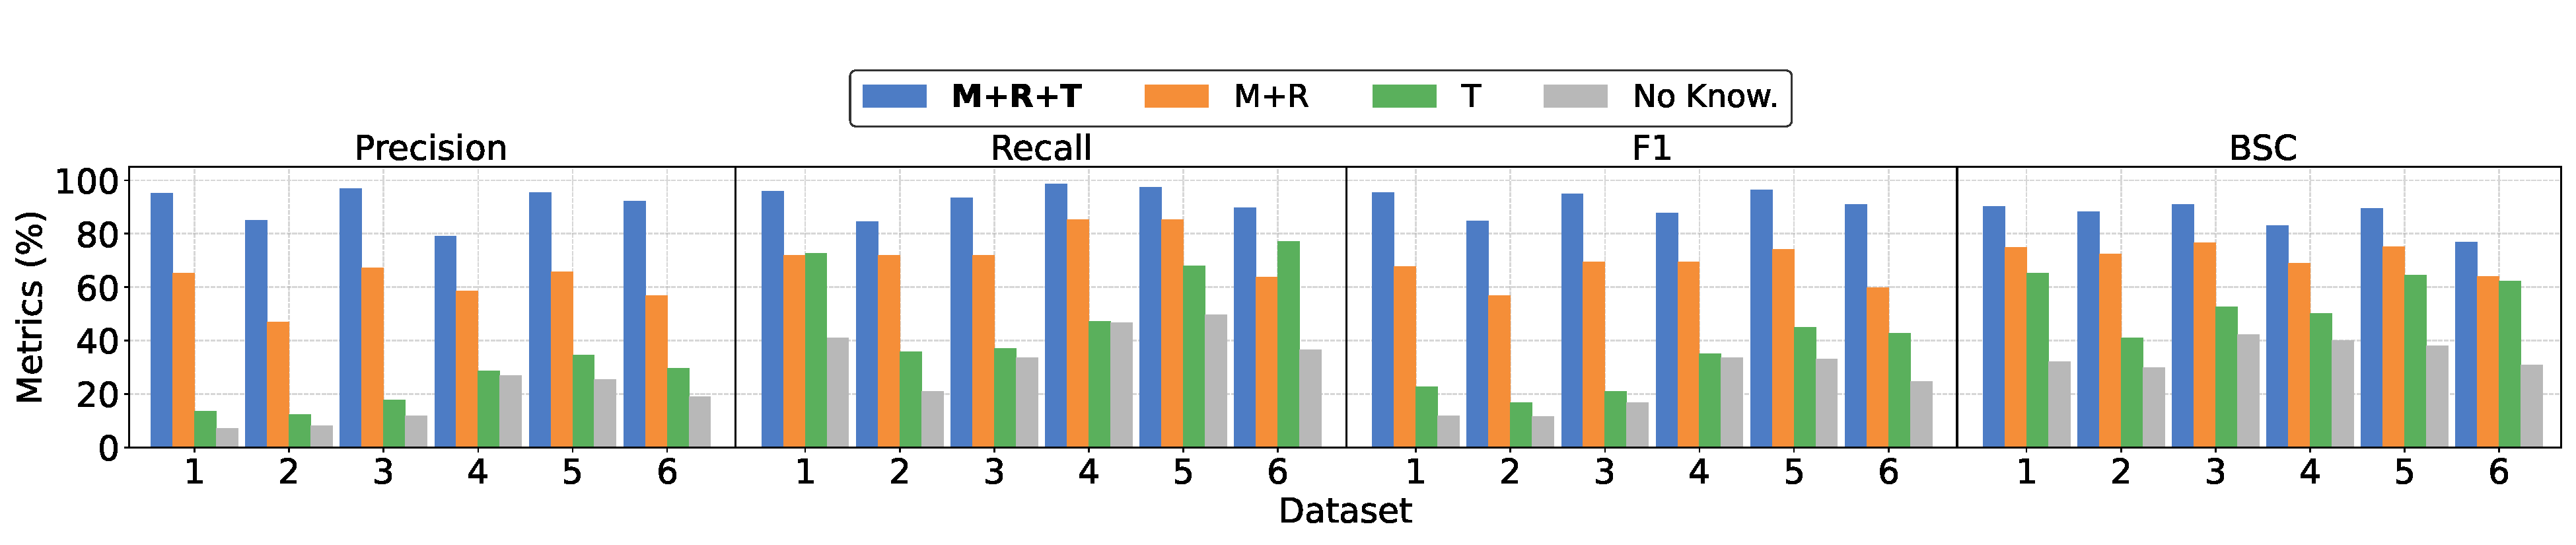
\includegraphics[width=\linewidth]{fig/exp2_all_metrics.pdf}
    \caption{Generated-test impact of valid knowledge bundles. $\mathcal{M}{+}\mathcal{R}$ is coupled because $\mathcal{R}$ is defined over $\mathcal{M}$; ``No Know.'' removes only explicit artifacts.}
    \label{fig:exp2}
    \Description{Four grouped bar charts compare Precision, Recall, F1, and BSC for full RAFT and three knowledge-ablation variants on six datasets. Full RAFT is highest throughout.}
\end{figure*}

\begin{figure*}[!t]
    \centering
    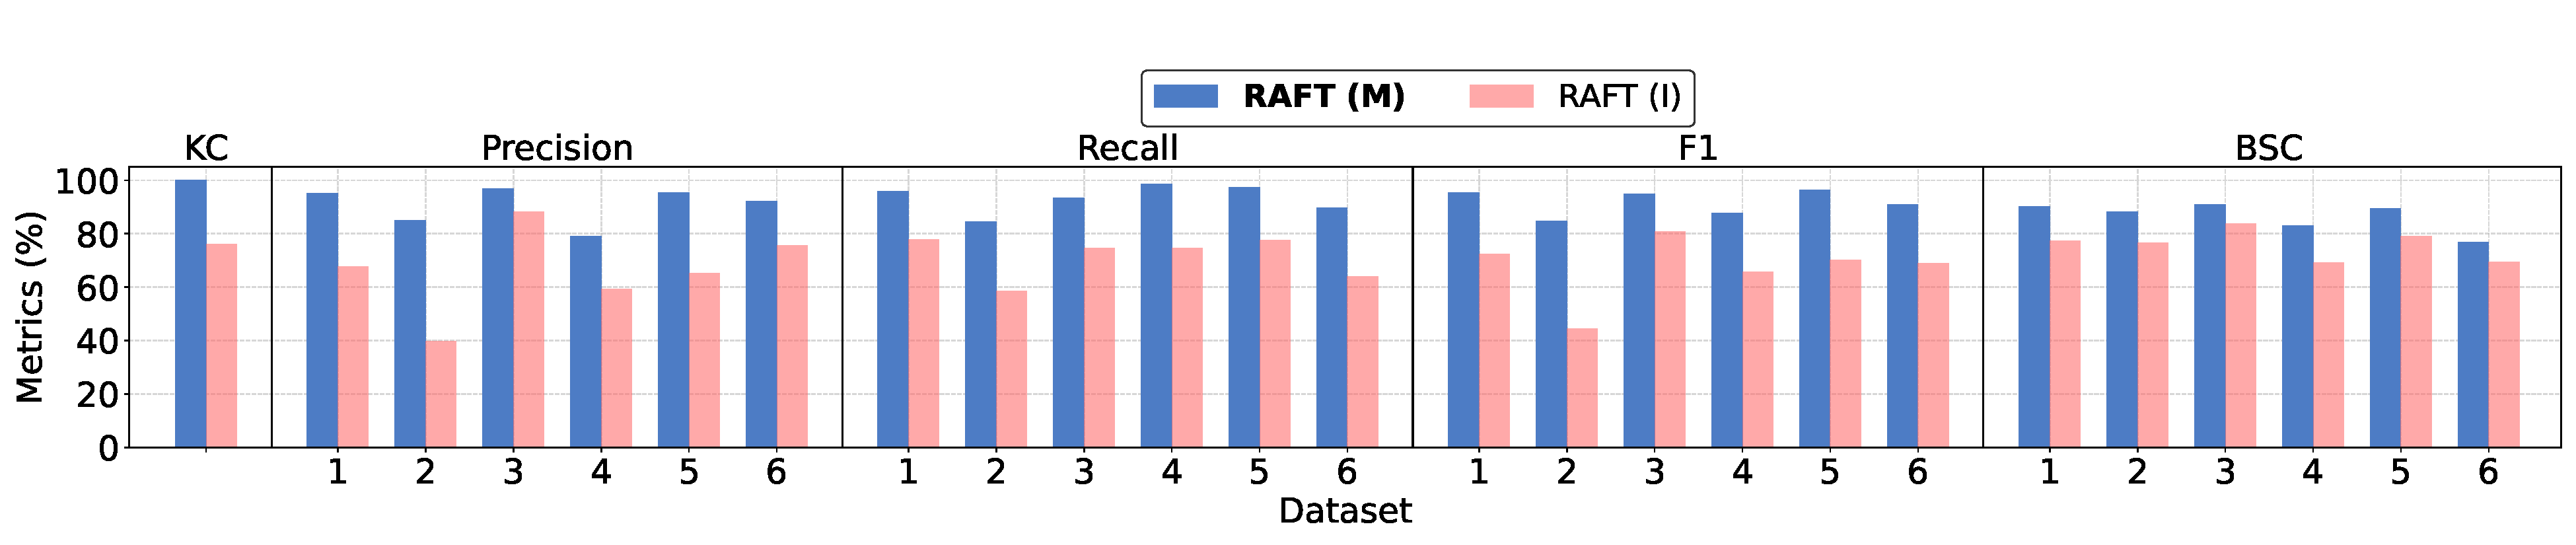
\includegraphics[width=\linewidth]{fig/exp2_2.pdf}
    \caption{Comparison of \ourtool\ using the \strategy\ strategy (\ourtool\ (M)) versus individual LLMs (\ourtool\ (I)). Knowledge coverage (KC) is the percentage of expert-consensus knowledge elements recovered; the remaining measures evaluate generated tests.}
    \label{fig:exp2_2}
    \Description{Grouped bar charts compare multi-LLM and individual-LLM RAFT for knowledge coverage, Precision, Recall, F1, and BSC. The multi-LLM setting is higher in every comparison.}
\end{figure*}

Fig.~\ref{fig:exp2_2} further shows that the individual-LLM variants have
23.9\% lower knowledge coverage, 26.8\% lower F1, and 12.2\% lower BSC on
average than the multi-LLM setting. This result shows the value of
consolidating multiple candidates; the operator analysis below tests whether
the proposed artifact-specific assignment preserves this gain downstream.

\begin{table*}[!t]
    \setlength{\tabcolsep}{5pt}
    \caption{Construction-source analysis on the six financial datasets. Each fidelity or coverage cell reports mean $\pm$ run-level standard deviation; within each run, results are macro-averaged across the six datasets and three LLM backends. Human effort measures the total person-hours required to construct and reconcile the knowledge artifacts and excludes downstream generation time.}
    \label{tab:exp2_source}
    \centering
    \resizebox{\linewidth}{!}{
    \begin{tabular}{lcccrrrrr}
        \toprule
        \textbf{Setting} &
        \textbf{\makecell{Construction\\Corpus}} &
        \textbf{\makecell{Explicit\\Artifacts}} &
        \textbf{Artifact Source} &
        \textbf{\makecell{Human Effort\\(person-h)}} &
        \textbf{Pre. (\%)} &
        \textbf{Rec. (\%)} &
        \textbf{F1 (\%)} &
        \textbf{BSC (\%)} \\
        \midrule
        \ourtool\ w/o Corpus & No & $\mathcal{M}{+}\mathcal{R}{+}\mathcal{T}$ & Multi-LLM & 0 & 82.8 $\pm$ 1.8 & 82.7 $\pm$ 2.1 & 82.7 $\pm$ 2.0 & 78.8 $\pm$ 1.7 \\
        Full-Corpus Prompting & Yes & None & -- & 0 & 62.6 $\pm$ 1.3 & 62.5 $\pm$ 1.2 & 62.5 $\pm$ 1.3 & 58.5 $\pm$ 1.2 \\
        \ourtool & Yes & $\mathcal{M}{+}\mathcal{R}{+}\mathcal{T}$ & Multi-LLM & 0 & 90.6 $\pm$ 6.7 & 93.0 $\pm$ 3.8 & 91.7 $\pm$ 4.3 & 87.1 $\pm$ 6.5 \\
        \ourtool\ w/ Expert Artifacts & Yes & $\mathcal{M}{+}\mathcal{R}{+}\mathcal{T}$ & Experts & 24.37 & 94.0 $\pm$ 3.0 & 93.9 $\pm$ 3.4 & 94.0 $\pm$ 3.2 & 91.2 $\pm$ 3.8 \\
        \bottomrule
    \end{tabular}
    }
\end{table*}

Table~\ref{tab:exp2_source} supports three controlled comparisons.
Without any construction corpus, \ourtool\ still reaches 82.7\% F1 and 78.8\%
BSC, retaining 90.2\% and 90.5\% of the full method's scores after all document
and historical-test cues are removed from artifact construction. This is
operational evidence that LLM parametric knowledge can induce useful
meta-level artifacts without an external construction corpus; it does not
imply that rule-specific semantics are recovered without reading the held-out
regulations in Phase~II. Adding the corpus raises F1 by 9.0 points and BSC by
8.3 points by providing additional evidence about expected content,
abstraction, terminology, and format.

\textit{Full-Corpus Prompting}
has access to the same corpus as \ourtool\ but trails it by 29.2 F1 points and
28.6 BSC points, indicating that transforming available knowledge into
structured artifacts contributes beyond placing the same corpus directly in
the generation context.

Expert-constructed artifacts add
only 2.3 F1 points and 4.1 BSC points over automatic explication but require 24.37
person-hours. Thus, the automatically explicated artifacts approach the
reference-case fidelity achieved by expert-constructed artifacts while
eliminating manual \emph{artifact-construction} effort;
this does not include evaluation or optional HITL review.

\begin{table*}[!t]
    \setlength{\tabcolsep}{10pt}
    \caption{End-to-end consolidation-operator assignment and hyperparameter sensitivity. Pur.\ and Agg.\ denote $K$-consensus purification and union-based aggregation, respectively. Artifact-quality cells report Precision/Recall (\%) against the expert-consensus artifacts; downstream F1 and BSC report mean $\pm$ run-level standard deviation. The $N=2$ setting is averaged over all three LLM pairs.}
    \label{tab:exp2_strategy}
    \centering
    \resizebox{\linewidth}{!}{
    \begin{tabular}{lccccccccrr}
        \toprule
        \textbf{Setting} &
        \textbf{$N$} & \textbf{$K$} &
        \textbf{$\mathcal{M}$} &
        \textbf{$\mathcal{R}$} &
        \textbf{$\mathcal{T}$} &
        \textbf{\makecell{$\mathcal{M}$ P/R\\(\%)}} &
        \textbf{\makecell{$\mathcal{R}$ P/R\\(\%)}} &
        \textbf{\makecell{$\mathcal{T}$ P/R\\(\%)}} &
        \textbf{F1 (\%)} &
        \textbf{BSC (\%)} \\
        \midrule
        All Purification & 3 & 2 & Pur. & Pur. & Pur. & 98.9/93.0 & 100.0/66.7 & 100.0/66.0 & 84.4 $\pm$ 2.8 & 78.6 $\pm$ 1.1 \\
        All Aggregation & 3 & -- & Agg. & Agg. & Agg. & 83.1/98.0 & 73.6/94.7 & 68.1/96.0 & 87.1 $\pm$ 2.7 & 79.9 $\pm$ 1.7 \\
        Reversed & 3 & 2 & Agg. & Pur. & Pur. & 83.1/98.0 & 100.0/71.3 & 100.0/69.0 & 85.2 $\pm$ 2.8 & 78.7 $\pm$ 2.6 \\
        \ourtool & 3 & 2 & Pur. & Agg. & Agg. & 98.9/93.0 & 83.6/92.0 & 72.7/96.0 & 91.7 $\pm$ 4.3 & 87.1 $\pm$ 6.5 \\
        \midrule
        \ourtool\ (Pairwise) & 2 & 2 & Pur. & Agg. & Agg. & 99.6/87.0 & 88.1/85.8 & 78.6/81.0 & 86.0 $\pm$ 2.1 & 79.3 $\pm$ 2.5 \\
        \ourtool\ (Strict) & 3 & 3 & Pur. & Agg. & Agg. & 100.0/84.0 & 83.4/90.7 & 71.4/90.0 & 87.2 $\pm$ 1.5 & 79.4 $\pm$ 1.2 \\
        \bottomrule
    \end{tabular}
    }
\end{table*}

Table~\ref{tab:exp2_strategy} shows the same trade-off at artifact and pipeline
levels. All Purification raises precision but reduces
$\mathcal{R}$/$\mathcal{T}$ recall to 66.7\%/66.0\%, yielding 84.4\% F1. All
Aggregation retains 94.7\%/96.0\% recall but propagates structural noise,
yielding 87.1\% F1; Reversed reaches 85.2\%. \ourtool's assignment retains
98.9\% $\mathcal{M}$ precision and 92.0\%/96.0\%
$\mathcal{R}$/$\mathcal{T}$ recall, producing the highest F1 (91.7\%) and BSC
(87.1\%). Two LLMs and unanimity lower downstream F1 to 86.0\% and 87.2\%,
respectively; these variants were preplanned and did not tune the default.

\noindent\textbf{Answer to RQ2.}
Corpus-free LLM-derived artifacts provide a strong starting point (82.7\% F1);
the corpus-supported workflow reaches 91.7\%. Purifying $\mathcal{M}$ and
aggregating $\mathcal{R}$ and $\mathcal{T}$ yields 4.6--7.3 more F1 points than
the alternative operator assignments after regenerating their dependent
artifacts and tests. Evaluation regulations remain the source of rule-specific semantics.
The ablation evaluates coupled $\mathcal{M}{+}\mathcal{R}$ and $\mathcal{T}$
rather than individual $\mathcal{M}$ or $\mathcal{R}$ effects.





\subsection{Experiment III: Step-Level Performance}
\label{sec:exp3}

\noindent
\textbf{Experimental Design.}
Experiment~III localizes the residual end-to-end errors observed in
Experiment~I. On the same six datasets, we compare one-shot requirements
generation (G Only) with up to three G-V-R repair iterations, and compare
natural-language (NL Cons.) with OCL-style testability criteria (OCL Cons.).
The latter are deterministic renderings of the same frozen five predicates,
with identical scope, polarity, exceptions, labels, and order. Two experts
verify their semantic correspondence; all other inputs and settings remain
fixed.

\noindent\textbf{Gold-Standard Construction.}
Before any run, two experts independently derive requirements and testability
labels from the source rules under a fixed guide and without model outputs.
They encode atomic obligations, conditions, exceptions, and outcomes as
\textit{KEY-OP-VALUE} with evidence and
\textit{Status}/\textit{ResultStatus}. Disagreements are resolved against the
source, followed by an omission check; the resulting versioned gold set is
frozen, hidden, and reused unchanged. The one-to-many rule mapping explains
Table~\ref{tab:exp1_dataset}. Requirements and labeled testability decisions
use the same maximum one-to-one set matching: unmatched generated items are
FPs, unmatched gold items are FNs, and a field or label mismatch leaves both
items unmatched, yielding one FP and one FN. Time and prompt/completion tokens
are also reported.

\begin{table}[!t]
    \setlength{\tabcolsep}{15pt}
    \caption{Step-level evaluation against the expert-constructed gold standard frozen before any model variant is run. The same gold set is used for every variant. Fidelity and classification metrics are macro-averaged across the six financial datasets; time and tokens are totals for processing all six.}
    \label{tab:exp3_}
    \centering
    \resizebox{\linewidth}{!}{
    \begin{tabular}{|c|c|ccc|c|cc|}
    \hline
    \textbf{Step} & \textbf{Variant} & \textbf{Pre. (\%)} & \textbf{Rec. (\%)} & \textbf{F1 (\%)} & \textbf{Time (m)} & \textbf{PTok} & \textbf{CTok} \\
        \hline
        \multirow{2}{*}{\makecell{\textbf{Requirements}\\\textbf{Generation}}} & G Only & 79.6 & 75.3 & 77.4 & 12.5 & 68,214 & 318,146\\
        \cline{2-8}
         & G-V-R & 91.6 & 87.7 & 89.0 & 34.9 & 210,247 & 982,237\\
        \hline
        \multirow{2}{*}{\makecell{\textbf{Testability}\\\textbf{Determination}}} & NL Cons. & 69.4 & 77.1 & 73.0 & 15.8 & 318,104 & 1,028,132\\
        \cline{2-8}
         & OCL Cons. & 96.2 & 95.5 & 95.8 & 14.6 & 436,159 & 938,117\\
        \hline
    \end{tabular}
    }
    \vspace{-2mm}
\end{table}


\noindent
\textbf{Experimental Results.}
Table~\ref{tab:exp3_} shows that G-V-R raises requirements-generation F1 from
77.4\% to 89.0\% (+11.6 points), primarily through a 12.0-point precision
gain. The repair loop adds 22.4 minutes, 142,033 prompt tokens, and 664,091
completion tokens over all six datasets. This is a measurable trade-off rather
than a free gain: G-V-R improves correctness, but omitted, incorrect, and
redundant elements remain and can propagate to final tests.

For testability determination, OCL Cons. raises F1 from 73.0\% to 95.8\%
(+22.8 points) while taking 1.2 fewer minutes. It uses 118,055 more prompt tokens
but 90,015 fewer completion tokens, leaving total token usage comparable. The
improvement in both Precision and Recall indicates that OCL-style serialization
presents the same scopes and predicates more consistently to the model than
their natural-language rendering.

Some errors are inherited from imperfect input requirements. The reported
testability score should therefore be interpreted as conditional on the
correctness of its input requirement.

% Since neither step is error-free, \ourtool\ supports a human-in-the-loop where experts correct the intermediate results. 
% As shown in Experiment~I, this intervention pushes \ourtool\ past expert-level performance with even less effort.




\noindent\textbf{Answer to RQ3.}
G-V-R improves requirements-generation F1 by 11.6 points to 89.0\%.
Representing the same testability predicates in OCL-style rather than
natural-language form improves testability F1 by 22.8 points to 95.8\%.



\subsection{Experiment IV: Sensitivity to LLM Backbone}
\label{sec:exp4}

\noindent
\textbf{Experimental Design.}
Experiment~IV addresses RQ4 by replacing the default backends with 11
open-weight LLMs spanning 2B--1.04T total parameters (Table~\ref{tab:exp4_llm}).
We report provider-stated total parameter counts only to describe and order the
tested backbones. The models also differ in architecture, training data, and
context length, so this experiment measures practical sensitivity to backbone
choice rather than the causal effect of parameter count or a scaling threshold.

Because each setting contains one LLM, that LLM independently explicates three
candidate versions of each artifact; \strategy\ then consolidates them before
the same LLM generates tests. The paired E2E baseline uses that model to
generate tests directly without \ourtool, while retaining the same evaluation
documents, output fields, matcher, and run protocol. On the six financial
datasets, we repeat each complete configuration three times and report mean F1;
the run-level minimum and maximum indicate variability. These models are
accessed through the OpenRouter endpoints listed in the replication package,
rather than a common local inference stack, so runtime and quantization are not
controlled or compared.

\begin{table}[!t]
    \setlength{\tabcolsep}{18pt}
    \caption{Open-weight LLMs used in the backbone-sensitivity analysis. Parameter counts are provider-reported total parameters used for descriptive ordering only; a dash indicates an undisclosed training cutoff.}
    \label{tab:exp4_llm}
    \centering
    \resizebox{\linewidth}{!}{
    \begin{tabular}{|c|c|c|c|c|}
    \hline
    \textbf{LLM} & \textbf{Total Params} & \textbf{Provider} & \textbf{Training Cutoff} & \textbf{Context Length} \\
        \hline
        Qwen3.5-2B \cite{qwen35_2b} & 2B & Alibaba & -- & 256K \\
        Gemma3-4B \cite{kamath2025gemma} & 4B & Google & 2024.08 & 128K \\
        Qwen3-4B \cite{yang2025qwen3} & 4B & Alibaba & - & 32K \\
        Gemma3-12B \cite{kamath2025gemma} & 12B & Google & 2024.08 & 128K \\
        GPT-OSS-20B \cite{agarwal2025gpt} & 21B & OpenAI & 2024.06 & 128K \\
        Gemma3-27B \cite{kamath2025gemma} & 27B & Google & 2024.08 & 128K \\
        Llama3.3-70B \cite{llama33} & 70B & Meta & 2023.12 & 128K \\
        GPT-OSS-120B \cite{agarwal2025gpt} & 117B & OpenAI & 2024.06 & 128K \\
        GLM4.5 \cite{zeng2025glm} & 355B & Zhipu AI & -- & 128K \\
        Llama3.1-405B \cite{grattafiori2024llama} & 405B & Meta & 2023.12 & 128K \\
        KimiK2 \cite{team2025kimi} & 1.04T & Moonshot AI & - & 256K \\
        \hline
    \end{tabular}
    }
\end{table}

\begin{figure}[!t]
    \centering
    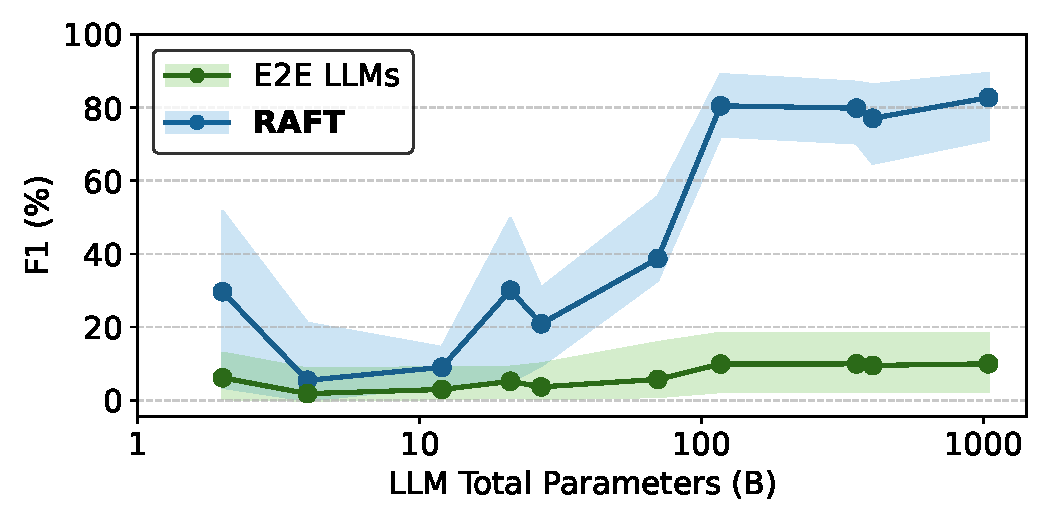
\includegraphics[width=0.6\linewidth]{fig/exp4.pdf}
    \caption{F1 for the tested LLM backbones, ordered by provider-reported total parameter count, for \ourtool\ and direct E2E generation. Lines denote three-run means and shaded regions denote run-level minima and maxima; the ordering does not identify a causal parameter-count effect.}
    \label{fig:exp4}
    \Description{A log-scale line chart orders tested backbones by provider-reported total parameter count. RAFT F1 varies substantially across models, while direct E2E generation remains near or below 10 percent for most models.}
\end{figure}


\noindent
\textbf{Experimental Results.}
Fig.~\ref{fig:exp4} reveals strong backbone dependence. Among the tested
models, those below 100B total parameters vary from near-zero to 38.7\% mean F1,
while the four selected models above 100B cluster at
76\%--83\%. This sampled pattern establishes neither a 100B threshold nor a
causal scaling relationship, and run ranges vary across backbones.

\ourtool\ exceeds the paired E2E baseline for 10 of the 11 models. The gap
varies across backbones, while direct generation remains near or below 10\% F1
for most tested models. Non-monotonic results among similarly sized models
reinforce that parameter count, architecture, training data, context length, and
provider runtime remain confounded.

Within-backbone gaps are more informative than cross-backbone ordering. Each
pair fixes the backbone, documents, schema, and matcher, but not calls or
tokens; it therefore evaluates the complete staged workflow rather than an
isolated artifact effect.


\noindent\textbf{Answer to RQ4.}
\ourtool\ improves over direct generation for 10 of 11 models, but remains
backbone-dependent; the experiment establishes neither a parameter threshold
nor a causal scaling effect.















\subsection{Experiment V: Cross-Domain Workflow Re-instantiation}
\label{sec:exp5}

\noindent
\textbf{Experimental Design.}
Experiment~V uses three road-traffic and two power-system datasets
(Table~\ref{tab:exp5_dataset}). Each pairs a cited official document with
pre-existing industry-authored reference cases, created independently of
\ourtool, source-checked, and frozen before evaluation. We retain the cited
language and edition and normalize only field names. Each family builds a
separate corpus; prompts, $N=3$, $K=2$, downstream procedure, metrics, schemas,
and operators remain fixed, and no financial artifact is reused.

\begin{table}[!t]
    \setlength{\tabcolsep}{15pt}
    \caption{Details of the five road-traffic and power-system evaluation datasets in Experiment V.}
    \label{tab:exp5_dataset}
    \centering
    \resizebox{\linewidth}{!}{
    \begin{tabular}{|c|c|p{5cm}|c|c|c|}
    \hline
    \textbf{Dataset} & \textbf{Domain} & \textbf{Document} & \textbf{\# Rule} & \textbf{\# Req.} & \textbf{\# TC} \\
        \hline
        \multirow{1}{*}{7} & \multirow{3}{*}{Road Traffic} & 2025 New Jersey Driver Manual \cite{dataset7} & \multirow{1}{*}{47} & \multirow{1}{*}{427} & \multirow{1}{*}{1570} \\
        \cline{1-1}\cline{3-6}
        \multirow{1}{*}{8} & & Road Traffic Safety Law of PRC \cite{dataset8} & \multirow{1}{*}{171} & \multirow{1}{*}{613} & \multirow{1}{*}{2124} \\
        \cline{1-1}\cline{3-6}
        \multirow{1}{*}{9} & & Cambodian Road Traffic Law \cite{dataset9} & \multirow{1}{*}{93} & \multirow{1}{*}{808} & \multirow{1}{*}{3132} \\
        \hline
        \multirow{1}{*}{10} & \multirow{2}{*}{Power} & EN 50549-1:2019 \cite{dataset10} & \multirow{1}{*}{75} & \multirow{1}{*}{362} & \multirow{1}{*}{703} \\
        \cline{1-1}\cline{3-6}
        \multirow{1}{*}{11} & & GB/T 19964-2024 \cite{dataset11} & \multirow{1}{*}{189} & \multirow{1}{*}{195} & \multirow{1}{*}{1311} \\
        \hline
    \end{tabular}
    }
\end{table}

\begin{figure}[!t]
    \centering
    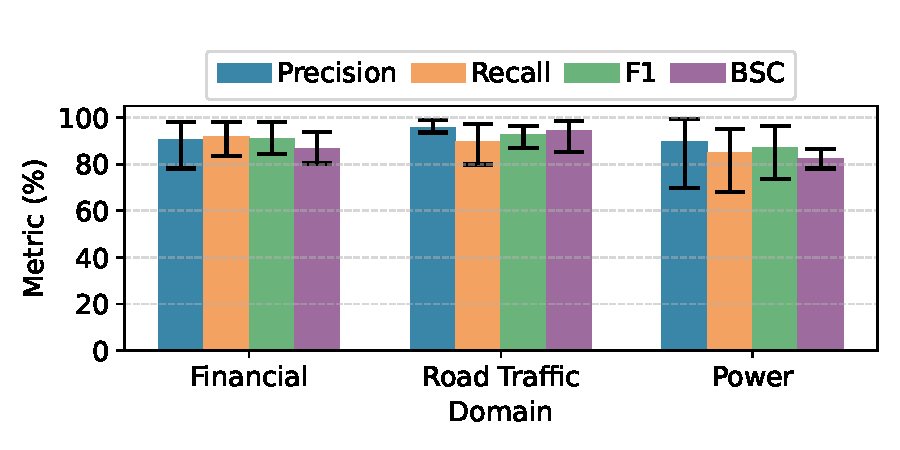
\includegraphics[width=0.5\linewidth]{fig/exp3.pdf}
    \caption{Family-level metric means; error bars show minimum and maximum dataset means.}
    \label{fig:exp5}
    \Description{A grouped bar chart shows Precision, Recall, F1, and BSC in the financial, road-traffic, and power-system document domains, with the power-system means lower and more variable.}
    \vspace{-2mm}
\end{figure}

\noindent
\textbf{Experimental Results.}
Road-traffic F1/BSC is 92.7\%/94.3\%, versus 91.7\%/87.1\% in finance;
power performance is 87.2\%/82.3\% (Fig.~\ref{fig:exp5}). Without domain
baselines, these differences are descriptive. Relative to finance, road traffic
is 1.0 F1 and 7.2 BSC points higher, whereas power is 4.5 F1 and 4.8 BSC points
lower. The error-bar ranges further show variation among documents within each
family; five non-financial datasets cannot establish broad domain superiority.

\noindent\textbf{Answer to RQ5.}
The workflow transfers after domain-specific re-instantiation while retaining
its artifact types and downstream protocol; the evidence does not establish
zero-shot portability.




\subsection{Threats to Validity}

\noindent
\textbf{Internal Validity.}
LLM stochasticity and baseline reimplementation remain; matched E2E runs,
ablations, paired operator settings with common source inputs and run seeds,
and common NL/OCL predicates reduce confounding. Each operator setting
regenerates dependent artifacts and tests, so its comparison is end-to-end.

\noindent
\textbf{Construct Validity.}
Incomplete reference cases and matcher errors mean F1/BSC measure fidelity, not
exhaustive validity or fault detection. Corpus-free does not remove parametric
knowledge; $\mathcal{M}{+}\mathcal{R}$ is coupled, and expert groups differ.
Residual subjectivity remains despite over 90\% initial agreement and
source-grounded reconciliation.

\noindent
\textbf{External Validity.}
Only five of 11 documents are outside finance, all reference cases are industrial, and
no domain baselines exist; evidence is limited to the evaluated documents.

\noindent
\textbf{Conclusion Validity.}
Six pairs provide limited power; corrected tests establish neither significance
nor expert equivalence. Experiment~IV establishes sensitivity, not a parameter
threshold or causal scaling.







% \subsection{Experiment IV: Impact of LLMs}

% \noindent
% \textbf{Experimental Design.}
% This experiment investigates how the capability of the underlying LLM affects knowledge extraction for constructing the meta-model and testable requirements representations. We approximate model capability by parameter size, evaluating 12 advanced LLMs with 2B-1T parameters under two settings: (1) each LLM performs the task individually, and (2) LLMs are grouped into four sets of three similarly sized models for aggregation. We then compare the completeness of the constructed meta-model and requirements representations, where \emph{completeness} is the percentage of correctly extracted elements, symbols, syntax, and testability components relative to the methodology in the main text. Model details are provided in Appendix \ref{sec:app:exp3}.


% \begin{figure}
%     \centering
%     \begin{subfigure}{0.235\textwidth}
%         \centering
%         \includegraphics[width=\textwidth]{fig/exp3_metamodel_completion.png}
%         \caption{Meta-Model}
%         \label{fig:exp3_metamodel}
%     \end{subfigure}
%     \begin{subfigure}{0.235\textwidth}
%         \centering
%         \includegraphics[width=\textwidth]{fig/exp3_representation_completion.png}
%         \caption{Req. Representation}
%         \label{fig:exp3_representation}
%     \end{subfigure}
%     \caption{Impact of LLM parameter size on the completeness of extracted domain knowledge.}
%     \label{fig:exp3}
% \end{figure}


% \noindent
% \textbf{Experimental Result.}
% The evaluation results are shown in Figure \ref{fig:exp3}. As the number of parameters increases, the completeness of both the meta-model and requirements representation shows a clear upward trend, indicating that stronger LLMs produce higher quality knowledge extraction. Our multi-LLM aggregation approach achieves over 90\% completeness with LLMs exceeding 100B parameters, establishing a practical lower bound for our method. In contrast, individual LLMs follow a similar trend but exhibit greater variability, reflecting the influence of randomness. Across all parameter settings, the multi-LLM aggregation consistently outperforms individual LLMs, underscoring the effectiveness of aggregation.

% \noindent
% \textbf{Conclusion:}
% Stronger LLMs consistently produce higher-quality knowledge, and our approach achieves over 90\% completeness with a lower bound of LLMs with 100B parameters.


















% \subsection{Experiment IV: Accuracy of Our Testable Requirements Generation}
% \label{sec:exp4}



% \begin{table}
%     \setlength{\tabcolsep}{3pt}
%     \caption{The quality of generated structured requirements of our approach using different LLMs.}
%     \label{tab:exp4_req}
%     \centering
%     \resizebox{\linewidth}{!}{
%     \begin{tabular}{|c|ccccc|ccc|}
%     \hline
%     \multirow{2}{*}{\textbf{O. LLM}} & \multicolumn{5}{c|}{\textbf{Token-Wise}} & \multicolumn{3}{c|}{\textbf{Word-Wise}} \\
%     \cline{2-9}
%      & \textbf{Pre.} & \textbf{Rec.} & \textbf{F1} & \textbf{BLEU} & \textbf{Rouge} & \textbf{Pre.} & \textbf{Rec.} & \textbf{F1} \\
%     \hline
%     GPT-5 & 80.9 & 72.3 & 75.0 & 44.8 & 73.9 & 75.6 & 66.0 & 69.0 \\
%     Grok-4 & 89.5 & 84.3 & 86.0 & 70.5 & 86.0 & 87.8 & 81.4 & 83.6 \\
%     \rowcolor{red!10} DeepSeek-R1 & 91.6 & 87.7 & 89.0 & 76.8 & 89.9 & 89.8 & 85.3 & 86.8 \\
%     \hline
%     \end{tabular}
%     }
% \end{table}


% \begin{table}
%     \setlength{\tabcolsep}{3pt}
%     \caption{Comparison of the accuracy of testability determination of our approach using different LLMs.}
%     \label{tab:exp4_test}
%     \centering
%     \resizebox{\linewidth}{!}{
%     \begin{tabular}{|c|c|c|>{\columncolor{red!10}}c|}
%     \hline
%     \textbf{O. LLM} & \textbf{NL only 1-step} & \textbf{NL+Req. 1-step} & \textbf{NL+Req. 5-step} \\
%     \hline
%     GPT-5 & 59.6 & 72.9 & 82.1 \\
%     Grok-4 & 63.8 & 74.3 & 89.5 \\
%     DeepSeek-R1 & 55.5 & 67.0 & 91.3 \\
%     \hline
%     \end{tabular}
%     }
% \end{table}

% \noindent
% \textbf{Experiment Design.}
% We evaluate the performance of structured requirements generation and testability determination on the 19 financial regulatory documents. Based on the financial metamodel and requirements representation, structured requirements are generated by the three LLMs and compared against manually constructed ground truth. The quality is evaluated using token-level metrics (Precision, Recall, F1, BLEU \cite{papineni2002bleu}, and ROUGE \cite{lin2004rouge}) and word-level metrics (precision, recall, and F1). We further assess downstream testability determination under three settings: (1) using natural language only; (2) using natural language with structured requirements and evaluating all criteria in a single step; and (3) using natural language with structured requirements in a five-step process, where each step evaluates one testability criterion. Precision, Recall, and F1 are reported relative to the ground-truth labels.

% \noindent
% \textbf{Experimental Result.}
% As shown in Table~\ref{tab:exp4_req}, our approach achieves consistently high accuracy in generating structured requirements across different LLMs, as reflected by strong token-level and word-level evaluation metrics. Among the evaluated models, DeepSeek-R1 attains the highest overall performance, indicating more accurate and stable structured requirements generation. 
% Table~\ref{tab:exp4_test} shows that using structured requirements leads to more accurate testability determination than relying on natural-language rules alone. In addition, the multi-step determination strategy consistently outperforms the one-step setting across all LLMs, suggesting that decomposing testability assessment into finer-grained steps yields more reliable results.

% \noindent
% \textbf{Conclusion:}
% Our approach is able to generate high-quality, testable structured requirements, providing a solid foundation for subsequent test generation.

\section{Conclusion}
\label{sec:conclusion}


\ourtool\ explicates implicit regulatory knowledge as a domain meta-model,
requirements representation, and testability constraints while keeping
regulations authoritative. Its seven-stage framework consolidates these
artifacts to formalize rules, assess testability, and generate traceable
compliance test cases. Across six financial datasets, \ourtool\ reaches 91.7\%
F1/87.1\% BSC, and HITL reaches 96.2\% F1. Ablations support explicit artifacts
and the artifact-specific assignment; backbone and cross-domain results show
sensitivity and re-instantiation rather than zero-shot generalization. Future
work will evaluate fault detection through system-specific execution and
broader domains.

% \section{Data Availability}
% An anonymized package, including code, prompts, and experimental datasets and results, is available at \url{https://github.com/1774531208/RAFT}. The repository will be made fully public upon acceptance.


\clearpage
\section{Data Availability}
An anonymized replication package containing our code, prompts, datasets,
ground truth, and results is available at
\url{https://github.com/1774531208/RAFT}.

\bibliographystyle{ACM-Reference-Format}
\bibliography{ref}

 % \clearpage
 % \appendix
 % \input{6_appendix}

\end{document}
